\documentclass[twoside,11pt,a4paper,openany]{book}
\usepackage[amsbb,subscriptcorrection,zswash,mtpcal,mtphrb]{mtpro2}
\usepackage[no-math,cm-default]{fontspec}
\usepackage{xunicode}
\usepackage{xgreek}
\defaultfontfeatures{Mapping=tex-text,Scale=MatchLowercase}
\def\xrwma{red!70!black}
\def\xrwmath{red!90!black}
\setmainfont[Mapping=tex-text,Numbers=Lining,Scale=1.0]{Minion Pro}
\newfontfamily\mpro{Minion Pro}
\usepackage{amsmath}
\usepackage[left=2.00cm, right=2.00cm, top=3.00cm, bottom=2.00cm]{geometry}
\usepackage{makeidx}
\usepackage{longtable}
\usepackage{etoolbox}
\makeatletter
\newif\ifLT@nocaption
\preto\longtable{\LT@nocaptiontrue}
\appto\endlongtable{%
\ifLT@nocaption
\addtocounter{table}{\m@ne}%
\fi}
\preto\LT@caption{%
\noalign{\global\LT@nocaptionfalse}}
\makeatother
\makeindex
\usepackage{tikz,pgfplots}
\usepackage{tkz-euclide,tkz-fct}
\usepackage{wrapfig}
\usetkzobj{all}
\usepackage{calc}
\usepackage{cleveref}
\usepackage[colorlinks=false, pdfborder={0 0 0}]{hyperref}
\usepackage[framemethod=TikZ]{mdframed}
\newcommand{\ypogrammisi}[1]{\underline{\smash{#1}}}
\usetikzlibrary{backgrounds}
\renewcommand{\thepart}{\arabic{part}}
\definecolor{steelblue}{cmyk}{.7,.278,0,.294}
\definecolor{doc}{cmyk}{1,0.455,0,0.569}
\definecolor{olivedrab}{cmyk}{0.25,0,0.75,0.44}
\usepackage{capt-of}
\usepackage{titletoc}
\usepackage[explicit]{titlesec}
\usepackage{graphicx}
\usepackage{multicol}
\usepackage{multirow}
\usepackage{enumitem}
\usepackage{tabularx}
\usepackage{mathimatika,tkz-tab,gensymb}
\usepackage[decimalsymbol=comma]{siunitx}
\tikzset{>=latex}
\makeatletter
\pretocmd{\@part}{\gdef\parttitle{#1}}{}{}
\pretocmd{\@spart}{\gdef\parttitle{#1}}{}{}
\makeatother
\usepackage[titletoc]{appendix}
\usepackage{fancyhdr}
\pagestyle{fancy}
\fancyheadoffset{0cm}
\renewcommand{\headrulewidth}{\iftopfloat{0pt}{.5pt}}
\renewcommand{\chaptermark}[1]{\markboth{#1}{}}
\renewcommand{\sectionmark}[1]{\markright{\it\thesection\ #1}}
\fancyhf{}
\fancyhead[LE]{\thepage\ $\cdot$\ \scshape\nouppercase{\leftmark}}
\fancyhead[RO]{\nouppercase{\rightmark} $\cdot$\ \thepage}
\fancypagestyle{plain}{%
\fancyhead{} %
\renewcommand{\headrulewidth}{0pt}}

\newcounter{thewrhma}[chapter]
\renewcommand{\thethewrhma}{\thechapter.\arabic{thewrhma}} 
\newcommand{\Thewrhma}[1]{\refstepcounter{thewrhma}{\textbf{\textcolor{\xrwmath}{{\large Θεώρημα\hspace{2mm}\thethewrhma\;}:\;}\hspace{1mm}}} \MakeUppercase{\textbf{#1}}\\}{}

\newcounter{porisma}[chapter]
\renewcommand{\theporisma}{\thechapter.\arabic{porisma}}\newcommand{\Porisma}[1]{\refstepcounter{porisma}\textcolor{black}{\textbf{ΠΟΡΙΣΜΑ\hspace{2mm}\theporisma\hspace{1mm} \MakeUppercase{#1}}}\\}{}

\newcounter{protasi}[chapter]
\renewcommand{\theprotasi}{\thechapter.\arabic{protasi}}\newcommand{\Protasi}[1]{\refstepcounter{protasi}\textcolor{black}{\textbf{ΠΡΟΤΑΣΗ\hspace{2mm}\theprotasi\hspace{1mm} \MakeUppercase{#1}}}\\}{}

\newcounter{methodologia}[chapter]
\renewcommand{\themethodologia}{\thechapter.\arabic{methodologia}}\newcommand{\Methodologia}[1]{\refstepcounter{methodologia}\textcolor{black}{\textbf{MΕΘΟΔΟΣ\hspace{2mm}\themethodologia\hspace{1mm} \MakeUppercase{#1}}}\\}{}

\newcounter{orismos}[chapter]
\renewcommand{\theorismos}{\arabic{orismos}}   
\newcommand{\Orismos}[1]{\refstepcounter{orismos}{\textbf{\textbf{\textcolor{\xrwma}{{\large Ορισμός\hspace{2mm}\thechapter.\theorismos\;}:\;}}}}\hspace{1mm} \MakeUppercase{\textbf{#1}\\}}{}
\usepackage{venndiagram}
%-------- ΣΤΥΛ ΚΕΦΑΛΑΙΟΥ ---------
\newcommand*\chapterlabel{}
\newcommand{\fancychapter}{%
\titleformat{\chapter}
{
\normalfont\Huge}
{\gdef\chapterlabel{\thechapter\ }}{0pt}
{\begin{tikzpicture}[remember picture,overlay]
\node[yshift=-7cm] at (current page.north west)
{\begin{tikzpicture}[remember picture, overlay]
%\node[inner sep=0pt] at ($(current page.north) +			(0cm,-1.38in)$) {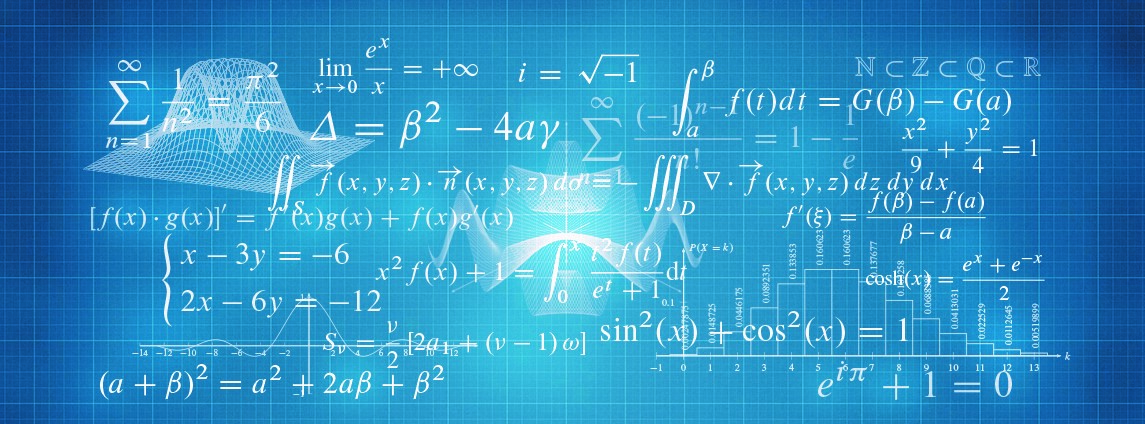
\includegraphics[width=17cm]{Kefalaio}};
\node[anchor=west,xshift=.08\paperwidth,yshift=.1\paperheight,rectangle]
{{\color{white}\fontsize{30}{20}\textbf{\textcolor{black}{\contour{white}{ΚΕΦΑΛΑΙΟ}}}}};
\node[anchor=west,xshift=.07\paperwidth,yshift=.05\paperheight,rectangle] {\fontsize{27}{20} {\color{black}{{\textcolor{black}{\contour{white}{\sc##1}}}}}};
%\fill[fill=black] (12.2,2) rectangle (14.8,4.7);
\node[anchor=west,xshift=.77\paperwidth,yshift=.077\paperheight,rectangle]
{\fontsize{80}{20}\textbf{\textit{\contour{black}{\thechapter}}}};
\end{tikzpicture}
};
\end{tikzpicture}
}
\titlespacing*{\chapter}{0pt}{20pt}{30pt}
}
%------------------------------------------------

\usepackage[outline]{contour}
\newcommand{\regularchapter}{%
\titleformat{\chapter}[display]
{\normalfont\huge\bfseries}{\chaptertitlename\ \thechapter}{20pt}{\Huge##1}
\titlespacing*{\chapter}
{0pt}{-20pt}{40pt}
}

\apptocmd{\mainmatter}{\fancychapter}{}{}
\apptocmd{\backmatter}{\regularchapter}{}{}
\apptocmd{\frontmatter}{\regularchapter}{}{}

\titlespacing*{\section}
{0pt}{30pt}{0pt}
\usepackage{booktabs}
\usepackage{hhline}
\DeclareRobustCommand{\perthousand}{%
\ifmmode
\text{\textperthousand}%
\else
\textperthousand
\fi}

\newcounter{typos}[chapter]
\renewcommand{\thetypos}{T\arabic{typos}}   
\newcommand{\Typos}{\refstepcounter{typos}\textcolor{gray}{\textbf{\thetypos}}}{}


\contentsmargin{0cm}
\titlecontents{part}[-1pc]
{\addvspace{10pt}%
\bf\Large ΜΕΡΟΣ\quad }%
{}
{}
{\;\dotfill\;\normalsize\ Σελίδα}%
%------------------------------------------
\titlecontents{chapter}[0pc]
{\addvspace{30pt}%
\begin{tikzpicture}[remember picture, overlay]%
\draw[fill=black,draw=black] (-.3,.5) rectangle (3.7,1.1); %
\pgftext[left,x=0cm,y=0.75cm]{\color{white}\sc\Large\bfseries Κεφάλαιο\ \thecontentslabel};%
\end{tikzpicture}\large\sc}%
{}
{}
{\hspace*{-2.3em}\hfill\normalsize Σελίδα \thecontentspage}%
\titlecontents{section}[2.4pc]
{\addvspace{1pt}}
{\contentslabel[\thecontentslabel]{2pc}}
{}
{\;\dotfill\;\small \thecontentspage}
[]
\titlecontents*{subsection}[4pc]
{\addvspace{-1pt}\small}
{}
{}
{\ --- \small\thecontentspage}
[ \textbullet\ ][]

\makeatletter
\renewcommand{\tableofcontents}{%
\chapter*{%
\vspace*{-20\p@}%
\begin{tikzpicture}[remember picture, overlay]%
\pgftext[right,x=12cm,y=0.2cm]{\Huge\sc\bfseries \contentsname};%
\draw[fill=black,draw=black] (9.5,-.75) rectangle (12.5,1);%
\clip (9.5,-.75) rectangle (15,1);
\pgftext[right,x=12cm,y=0.2cm]{\color{white}\Huge\bfseries \contentsname};%
\end{tikzpicture}}%
\@starttoc{toc}}
\makeatother
\pgfmathdeclarefunction{gauss}{2}{%
\pgfmathparse{1/(#2*sqrt(2*pi))*exp(-((x-#1)^2)/(2*#2^2))}%
}
\usepackage[contents={},scale=1,opacity=1,color=black,angle=0]{background}

\newcommand\blfootnote[1]{%
\begingroup
\renewcommand\thefootnote{}\footnote{#1}%
\addtocounter{footnote}{-1}%
\endgroup
}
\usepackage{epstopdf}
\epstopdfsetup{update}
\usepackage{textcomp}
\titleformat{\section}
{\normalfont\Large\bf}%
{}{0em}%
{{\color{black}\titlerule[1pt]}\vskip-.2\baselineskip{\parbox[t]{\dimexpr\textwidth-2\fboxsep\relax}{\raggedright\strut\thesection~#1\strut}}}[\vskip 0\baselineskip{\color{black}\titlerule[1pt]}]
\titlespacing*{\section}{0pt}{0pt}{0pt}

\newcommand{\methodologia}{\begin{center}
{\large \textbf{ΜΕΘΟΔΟΛΟΓΙΑ}}\\\vspace{-2mm}
\begin{tikzpicture}
\shade[left color=white, right color=black] (-3cm,0) rectangle (0,.2mm);
\shade[left color=black, right color=white] (0,0) rectangle (3cm,.2mm);   
\end{tikzpicture}
\end{center}}

\newcommand{\orismoi}{\begin{center}
\large \textcolor{\xrwma}{\textbf{ΟΡΙΣΜΟΙ}}\\\vspace{-2mm}
\begin{tikzpicture}
\shade[left color=white, right color=\xrwma] (-3cm,0) rectangle (0,.2mm);
\shade[left color=\xrwma, right color=white] (0,0) rectangle (3cm,.2mm);   
\end{tikzpicture}
\end{center}}
\newcommand{\thewrhmata}{\begin{center}
{\large \textcolor{\xrwmath}{\textbf{ΘΕΩΡΗΜΑΤΑ - ΠΟΡΙΣΜΑΤΑ - ΠΡΟΤΑΣΕΙΣ\\ΚΡΙΤΗΡΙΑ - ΙΔΙΟΤΗΤΕΣ}}}\\\vspace{-2mm}
\begin{tikzpicture}
\shade[left color=white, right color=\xrwmath,] (-5cm,0) rectangle (0,.2mm);
\shade[left color=\xrwmath, right color=white,] (0,0) rectangle (5cm,.2mm);   
\end{tikzpicture}
\end{center}}
\usepackage[labelfont={footnotesize,it,bf},font={footnotesize}]{caption}

\usepackage{wrapfig,wrap-rl}
%-------- ΜΑΘΗΜΑΤΙΚΑ ΕΡΓΑΛΕΙΑ ---------
\usepackage{mathtools}
%----------------------
%-------- ΠΙΝΑΚΕΣ ---------
\usepackage{booktabs}
%----------------------
%----- ΥΠΟΛΟΓΙΣΤΗΣ ----------
%\usepackage{calculator}
%----------------------------
\newcommand{\tss}[1]{\textsuperscript{#1}}
\newcommand{\tssL}[1]{\MakeLowercase{\textsuperscript{#1}}}
%----- ΟΡΙΖΟΝΤΙΑ ΛΙΣΤΑ ------
\usepackage{xparse}
\newcounter{answers}
\renewcommand\theanswers{\arabic{answers}}
\ExplSyntaxOn
\NewDocumentCommand{\results}{m}
{
\seq_set_split:Nnn \l_results_a_seq {,}{#1}
\par\nobreak\noindent\setcounter{answers}{0}
\seq_map_inline:Nn \l_results_a_seq
{
\makebox[.18\linewidth][l]{\stepcounter{answers}\theanswers.~##1}\hfill
}
\par
}
\seq_new:N \l_results_a_seq
\ExplSyntaxOff
%----------------------------

\usepackage{microtype}
\usepackage{float}
\usepackage{caption}
%----------- ΓΡΑΦΙΚΕΣ ΠΑΡΑΣΤΑΣΕΙΣ ---------
\pgfkeys{/pgfplots/aks_on/.style={axis lines=center,
xlabel style={at={(current axis.right of origin)},xshift=1.5ex, anchor=center},
ylabel style={at={(current axis.above origin)},yshift=1.5ex, anchor=center}}}
\pgfkeys{/pgfplots/grafikh parastash/.style={\xrwma,line width=.4mm,samples=200}}
\pgfkeys{/pgfplots/belh ar/.style={tick label style={font=\scriptsize},axis line style={-latex}}}
%-----------------------------------------

%---- ΟΡΙΖΟΝΤΙΟ - ΚΑΤΑΚΟΡΥΦΟ - ΠΛΑΓΙΟ ΑΓΚΙΣΤΡΟ ------
\newcommand{\orag}[3]{\node at (#1)
{$ \overcbrace{\rule{#2mm}{0mm}}^{{\scriptsize #3}} $};}

\newcommand{\kag}[3]{\node at (#1)
{$ \undercbrace{\rule{#2mm}{0mm}}_{{\scriptsize #3}} $};}

\newcommand{\Pag}[4]{\node[rotate=#1] at (#2)
{$ \overcbrace{\rule{#3mm}{0mm}}^{{\rotatebox{-#1}{\scriptsize$#4$}}}$};}
%-----------------------------------------
\tikzstyle{pl}=[line width=0.3mm]
\tikzstyle{plm}=[line width=0.4mm]
\tkzSetUpPoint[size=7,fill=white]
\newlist{rlist}{enumerate}{3}
\setlist[rlist]{itemsep=0mm,label=\roman*.}
\setlist[itemize]{itemsep=0mm}
\definecolor{bblue}{HTML}{4F81BD}
\definecolor{rred}{HTML}{C0504D}
\definecolor{ggreen}{HTML}{9BBB59}
\definecolor{ppurple}{HTML}{9F4C7C}

\makeatletter
\usetikzlibrary{patterns}
\tikzstyle{chart}=[
legend label/.style={font={\scriptsize},anchor=west,align=left},
legend box/.style={rectangle, draw, minimum size=5pt},
axis/.style={black,semithick,->},
axis label/.style={anchor=east,font={\tiny}},
]

\tikzstyle{bar chart}=[
chart,
bar width/.code={
\pgfmathparse{##1/2}
\global\let\bar@w\pgfmathresult
},
bar/.style={very thick, draw=white},
bar label/.style={font={\bf\small},anchor=north},
bar value/.style={font={\footnotesize}},
bar width=.75,
]

\tikzstyle{pie chart}=[
chart,
slice/.style={line cap=round, line join=round,thick,draw=white},
pie title/.style={font={\bf}},
slice type/.style 2 args={
##1/.style={fill=##2},
values of ##1/.style={}
}
]

\pgfdeclarelayer{background}
\pgfdeclarelayer{foreground}
\pgfsetlayers{background,main,foreground}


\newcommand{\pie}[3][]{
\begin{scope}[#1]
\pgfmathsetmacro{\curA}{90}
\pgfmathsetmacro{\r}{1}
\def\c{(0,0)}
\node[pie title] at (90:1.3) {#2};
\foreach \v/\s/\l in{#3}{
\pgfmathsetmacro{\deltaA}{\v/100*360}
\pgfmathsetmacro{\nextA}{\curA + \deltaA}
\pgfmathsetmacro{\midA}{(\curA+\nextA)/2}

\path[slice,\s] \c
-- +(\curA:\r)
arc (\curA:\nextA:\r)
-- cycle;
\pgfmathsetmacro{\d}{max((\deltaA * -(.5/50) + 1) , .5)}

\begin{pgfonlayer}{foreground}
\path \c -- node[pos=\d,pie values,values of \s]{$\l$} +(\midA:\r);
\end{pgfonlayer}

\global\let\curA\nextA
}
\end{scope}
}

\newcommand{\legend}[2][]{
\begin{scope}[#1]
\path
\foreach \n/\s in {#2}
{
++(0,-10pt) node[\s,legend box] {} +(5pt,0) node[legend label] {\n}
}
;
\end{scope}
}
\definecolor{a}{cmyk}{0,1,1,0.05}
\definecolor{b}{cmyk}{0,.8,.8,.15}
\definecolor{c}{cmyk}{0,.8,.8,.0}
\definecolor{d}{cmyk}{0,.7,.7,0}
\definecolor{e}{cmyk}{0,.5,.5,0}


\pgfplotsset{every axis/.append style={
x tick label style={/pgf/number format/.cd, 1000 sep={.}}}}
\newcommand{\shmeio}[2]{
\foreach \a in {1,...,#2}{
\node[dot] at (#1+.5,\a/2-.2){};}}


\newfontfamily\scfont{GFS Artemisia}
\font\icon = "Webdings"
\font\icons = "IcoMoon-Free"
\font\myfont = "Wingdings"
\font\mymath = "MyMathSymbols" at 16pt
\newcommand{\titlos}[3]{
\begin{center}
{\large {\textcolor{\xrwma}{\scfont\textsc{Σπύρος}}\,\,\textcolor{\xrwma}{\scfont\textsc{Φρόνιμος}}} - {\scfont\textsc{Μαθηματικός}}}
\\{\myfont\XeTeXglyph13} : spyrosfronimos@gmail.com\,\,|\,\,{\icons\XeTeXglyph188} : 6932327283 - 6974532090\\
\rule{12.7cm}{.1mm}\\
\vspace{2mm}
ΣΗΜΕΙΩΣΕΙΣ ΘΕΩΡΙΑΣ - ΟΡΙΣΜΟΙ ΚΑΙ ΘΕΩΡΗΜΑΤΑ\\
\vspace{1mm}
{\bf\today}
\end{center}
\vspace{.5cm}
\begin{center}
{\Large\bf\MakeUppercase{#1}}
\end{center}
\begin{center}
\textbf{{\Huge \textcolor{\xrwma}{#2}}}
\end{center}
\vspace{-5mm}
\begin{center}
{\Large\bf{\MakeUppercase{#3}}}
\end{center}
\vspace{1cm}}









\begin{document}
\pagenumbering{gobble}% Remove page numbers (and reset to 1)
\clearpage
\backmatter
\pagestyle{empty}
\titlos{Α΄ ΓΥΜΝΑΣΙΟΥ}{Μαθηματικά}{Ορισμοί και θεωρήματα}
\vspace{1cm}
\begin{center}
\begin{tikzpicture}[scale=1.2]
\clip (-.5,-.5) rectangle (5.2,2.2);
\tkzDefPoint(0,0){A}
\tkzDefPoint(3,0){B}
\tkzDefPoint(2.5,1.7){C}
\draw (B) -- (A) -- (C);
\tkzDrawBisector[draw=\xrwma](B,A,C)\tkzGetPoint{a}
\tkzDefPointWith[linear,K=0.8](A,a) \tkzGetPoint{D}
\tkzDefPointBy[projection=onto A--C](D)
\tkzGetPoint{h}
\tkzDrawSegment(D,h)
\tkzMarkRightAngle[fill=\xrwma](A,h,D)
\tkzDefPointBy[projection=onto A--B](D)
\tkzGetPoint{f}
\tkzDrawSegment(D,f)
\tkzMarkRightAngle[fill=\xrwma](A,f,D)
\tkzLabelPoint[left](A){$A$}
\tkzLabelPoint[above,xshift=2mm](D){$M$}
\tkzLabelPoint[above](h){$B$}
\tkzLabelPoint[below](f){$\varGamma$}
\tkzLabelPoint[above](C){$y$}
\tkzLabelPoint[right](B){$x$}
\tkzDrawPoints(A,h,f,D)
\node at (4,.8){$ MB=M\varGamma $};
\end{tikzpicture}\mbox{}\\
\vspace{3cm}
\begin{minipage}{7cm}
\begin{center}
ΑΝΑΛΥΤΙΚΟ ΤΥΠΟΛΟΓΙΟ ΓΙΑ ΤΗ ΘΕΩΡΙΑ ΤΩΝ ΜΑΘΗΜΑΤΙΚΩΝ Α΄ ΓΥΜΝΑΣΙΟΥ
\end{center}
\end{minipage}
\end{center}
\vspace*{\fill{\begin{center}
\end{center}}}
\pagenumbering{arabic}
\mainmatter
\pagestyle{fancy}
\chapter{Αλγεβρικές Παραστάσεις}
\section{Φυσικοί Αριθμοί - Διάταξη - Στρογγυλοποίηση}\mbox{}\\
\orismoi
\Orismos{Φυσικοί Αριθμοί}
Φυσικοί ονομάζονται οι αριθμοί από το $ 0 $ έως το άπειρο όπου κάθε αριθμός έχει διαφορά μιας μονάδας από τον προηγούμενο.
\[ 0,1,2,3,4,5,\ldots \]
\Orismos{Άρτιοι - περιττοι αριθμοί}
Άρτιοι ή ζυγοί ονομάζονται οι φυσικοί αριθμοί που διαιρούνται με το $ 2 $ ενώ περιττοί ή μονοί όσοι δεν διαιρούνται με το $ 2 $. 
\begin{itemize}
\item Το τελευταίο ψηφίο κάθε άρτιου αριθμού είναι ένα από τα $ 0,2,4,6,8 $. 
\item Ένας περιττός αριθμός τελείώνει σε ένα από τα ψηφία $ 1,3,5,7,9 $.
\end{itemize}
\Orismos{Δεκαδικο συστημα αρίθμησης}
Δεκαδικό ονομάζεται το σύστημα αρίθμησης στο οποίο κάθε αριθμός σχηματίζεται με τη χρήση των δέκα συμβόλων - ψηφίων : $ 0,1,2,3,4,5,6,7,8,9 $ τοποθετημένα διαδοχικά το ένα μετά το άλλο. Καθένα απ' αυτά έχει διαφορετική αξία ανάλογα με το πλήθος των μονάδων που εκφράζει. Στο δεκαδικό σύστημα έχουμε σαν βάση τον αριθμό δέκα.
\begin{center}
\begin{longtable}{c|>{\centering\arraybackslash}m{1.5cm}|>{\centering\arraybackslash}m{1.5cm}|>{\centering\arraybackslash}m{1.2cm}|>{\centering\arraybackslash}m{1cm}|>{\centering\arraybackslash}m{1.5cm}|>{\centering\arraybackslash}m{1cm}|>{\centering\arraybackslash}m{1cm}}
\hline  \multicolumn{8}{c}{\textbf{Ψηφία Ακέραιου Αριθμού}} \rule[-2ex]{0pt}{5.5ex}\\ 
\hhline{========} \rule[-2ex]{0pt}{6ex} \begin{minipage}{1.5cm}
\begin{center}
{\footnotesize \textbf{Δεκαδική}}\\{\footnotesize \textbf{Τάξη}}
\end{center}
\end{minipage} &
{\footnotesize Εκατομμύρια} & 
\begin{minipage}{1.5cm}
\begin{center}
\vspace{-1.4mm}
{\footnotesize Εκατοντάδες}\\{\footnotesize Χιλιάδες}
\end{center}
\end{minipage} & 
\begin{minipage}{1.3cm}
\begin{center}
{\footnotesize Δεκάδες}\\{\footnotesize Χιλιάδες}
\end{center}
\end{minipage} & 
{\footnotesize Χιλιάδες}& 
{\footnotesize Εκατοντάδες} & 
{\footnotesize Δεκάδες}& 
{\footnotesize Μονάδες}  \\ 
\hline \rule[-1.5ex]{0pt}{4.5ex} {\footnotesize \textbf{Συμβ.}} & {\footnotesize Εκ} & {\footnotesize ΕΧ} & {\footnotesize ΔΧ} & {\footnotesize Χ} & {\footnotesize Ε} & {\footnotesize Δ} & {\footnotesize Μ} \\ 
\hline \rule[-1.5ex]{0pt}{4.5ex} {\footnotesize \textbf{Αξία}} & {\footnotesize $ 1.000.000 $} & {\footnotesize $ 100.000 $} & {\footnotesize $ 10.000 $} & {\footnotesize $ 1.000 $} & {\footnotesize $ 100 $} & {\footnotesize $ 10 $} & {\footnotesize $ 1 $}\\
\hline 
\end{longtable}
\end{center}
\begin{itemize}[itemsep=0mm]
\item Κάθε αριθμός έχει διαφορετική αξία ανάλογα με τη θέση και την αξία των ψηφίων που τον αποτελούν.
\item Σε κάθε αριθμό η θέση κάθε ψηφίου καθορίζει την αξία του. Η θέση αυτή ονομάζεται \textbf{δεκαδική θέση}.
\item Η αξία των δεκαδικών θέσεων αυξάνεται από τα δεξιά προς τα αριστερά.
\item Κάθε δεκαδική θεση έχει αξία δεκαπλάσια της προηγούμενης.
\end{itemize}
\Orismos{Διάταξη}
Διάταξη ονομάζεται η ιδιότητα του συνόλου των φυσικών αριθμών με την οποία μπορούμε να τους συγκρίνουμε και να τους τοποθετήσουμε σε σειρά από το μικρότερο στο μεγαλύτερο ή αντίστροφα. Τα σύμβολα διάταξης που χρησιμοποιούμε είναι:
\begin{center}
$ < $ : μικρότερο  \;,\;  $ > $ : μεγαλύτερο  \;,\; $ \leq $  μικρότερο ίσο \;,\; $ \geq $  μεγαλύτερο ισο  
\end{center}
\Orismos{Άξονασ των αριθμών}
Ο άξονας των φυσικών αριθμών είναι μια αριθμημένη ημιευθεία στην οποία μπορούν να τοποθετηθούν όλοι οι φυσικοί αριθμοί σε αύξουσα σειρά από τα αριστερά προς τα δεξιά.
\begin{center}
\begin{tikzpicture}
\tkzInit[xmin=0,xmax=4]
\draw[-latex] (0,0) -- coordinate (x axis mid) (4.4,0) node[right,fill=white] {{\footnotesize $ x $}};
\foreach \x in {0,...,4}
\draw (\x,.5mm) -- (\x,-.5mm) node[anchor=north,fill=white] {{\scriptsize \x}};
\tkzText(2,0.7){Φυσικοί Αριθμοί}
\tkzDefPoint(2,0){A}
\tkzDrawPoint(A)
\tkzLabelPoint[above](A){{\scriptsize $ A(2) $}}
\end{tikzpicture}
\end{center}
\begin{itemize}[itemsep=0mm]
\item \textbf{Αρχή} του άξονα είναι το σημείο στο οποίο βρίσκεται ο αριθμός $ 0 $.
\item Η θέση ενός αριθμού πάνω στην ευθεία σχεδιάζεται με ένα σημείο.
\item Ο αριθμός που βρίσκεται στη θέση αυτή ονομάζεται \textbf{τετμημένη} του σημείου.
\end{itemize}
\Orismos{Στρογγυλοποίηση}
Στρογγυλοποίηση ονομάζεται η διαδικασία με την οποία αντικαθιστούμε έναν αριθμό με έναν άλλον ο οποίος είναι μια πιο \textbf{απλή} προσέγγισή του. Η στρογγυλοποίηση ενός αριθμού γίνεται σε οποιοδήποτε ψηφίο του, το οποίο ονομάζεται \textbf{τάξη στρογγυλοποίησης}.
\section{Πρόσθεση, αφαίρεση και πολλ/μος φυσικών αριθμών}\mbox{}\\
\orismoi
\Orismos{Πράξεισ αριθμών}
Στον παρακάτω πίνακα φαίνονται τα ονόματα των αριθμών που αποτελούν μια πράξη, τα ονόματα των αποτελεσμάτων και ο συμβολισμός κάθε πράξης.
\begin{center}
\begin{tabular}{cccc}
\hline \rule[-2ex]{0pt}{5.5ex} \textbf{Πράξη} & \textbf{Όροι} & \textbf{Αποτέλεσμα} & \textbf{Συμβολισμός} \\ 
\hhline{====} \rule[-2ex]{0pt}{5.5ex} \textbf{Πρόσθεση} & Προσθετέοι & Άθροισμα & $ a+\beta $ \\ 
\rule[-2ex]{0pt}{5.5ex} \textbf{Αφαίρεση} & Μειωτέος - Αφαιρετέος & Διαφορά & $ a-\beta $ \\ 
\rule[-2ex]{0pt}{5.5ex} \textbf{Πολλαπλασιασμός} & Παράγοντες & Γινόμενο & $ a\cdot\beta $ \\ 
\hline\end{tabular}
\end{center}
\begin{enumerate}[itemsep=0mm,label=\bf\arabic*.]
\item \textbf{Πρόσθεση}\\ Πρόσθεση ονομάζεται η πράξη με την οποία μπορούμε από δύο αριθμούς $ a,\beta\in\mathbb{R} $ να υπολογίσουμε τον αριθμό $ a+\beta $ που ονομάζεται \textbf{άθροισμα}.
\item \textbf{Πολλαπλασιασμόσ}\\
Πολλαπλασιασμός ονομάζεται η πράξη με την οποία μπορούμε από δύο αριθμούς $ a,\beta $ να υπολογίσουμε τον αριθμό $ a\cdot\beta $ που ονομάζεται \textbf{γινόμενο}.
\item \textbf{Αφαίρεση - Διαίρεση}\\
Αφαίρεση ονομάζεται η πράξη με την οποία μπορούμε από δύο αριθμούς $ a $ και $ \beta $ να υπολογίσουμε τον αριθμό $ a-\beta $ η τον $ \beta-a $ ο οποίος ονομάζεται \textbf{διαφορά}.
\end{enumerate}
\thewrhmata
\Thewrhma{Ιδιότητεσ των Πράξεων}
Στον παρακάτω πίνακα βλέπουμε τις βασικές ιδιότητες της πρόσθεσης και του πολλαπλασιασμού στο σύνολο των πραγματικών αριθμών.
\begin{center}
\begin{tabular}{ccc}
\hline \rule[-2ex]{0pt}{5.5ex} \textbf{Ιδιότητα} & \textbf{Πρόσθεση} & \textbf{Πολλαπλασιασμός} \\ 
\hhline{===} \rule[-2ex]{0pt}{5.5ex} \textbf{Αντιμεταθετική} & $ a+\beta=\beta+a $ & $ a\cdot\beta=\beta\cdot a $ \\
\rule[-2ex]{0pt}{5ex} \textbf{Προσεταιριστική} & $ a+\left( \beta+\gamma\right) =\left( a+\beta\right) +\gamma $ & $ a\cdot\left( \beta\cdot\gamma\right) =\left( a\cdot\beta\right)\cdot\gamma $\\
\rule[-2ex]{0pt}{5ex} \textbf{Ουδέτερο στοιχείο} & $ a+0=a $ & $ a\cdot1= a $\\
\rule[-2ex]{0pt}{5ex} \textbf{Επιμεριστική} & \multicolumn{2}{c}{$ a\cdot\left( \beta\pm\gamma\right)=a\cdot\beta\pm a\cdot\gamma  $}\\
\hline
\end{tabular}
\end{center}
\section{Δυνάμεις φυσικών αριθμών}\mbox{}\\
\orismoi
\Orismos{Δύναμη φυσικού αριθμου}
Δύναμη ενός φυσικού αριθμού $ a $ ονομάζεται το γινόμενο $ \nu $ ίσων παραγόντων του αριθμού αυτού. Συμβολίζεται με $ a^\nu $ όπου $ \nu $ είναι το πλήθος των ίσων παραγόντων. 
\[ \undercbrace{a\cdot a\cdot\ldots a}_{\nu\textrm{ παράγοντες }}=a^\nu \]
\begin{itemize}[itemsep=0mm]
\item Ο αριθμός $ α $ ονομάζεται \textbf{βάση} και ο αριθμός $ \nu $ \textbf{εκθέτης} της δύναμης.
\item Η δύναμη $ a^2 $ ονομάζεται και $ \mathbold{a} $ \textbf{στο τετράγωνο}.
\item Η δύναμη $ a^3 $ ονομάζεται και  {\boldmath $ a $}  \textbf{στον κύβο}.
\end{itemize}
\Orismos{Αριθμητική παράσταση}
Αριθμητική ονομάζεται κλαθε παράσταση που περιέχει πράξεις μεταξύ φυσικών αριθμών. Η προτεραιότητα των πράξεω σε μια αριθμητική παράσταση είναι η εξής:
\begin{multicols}{2}
\begin{enumerate}[itemsep=0mm]
\item Δυνάμεις
\item Πολλαπλασιασμοί και διαιρέσεις
\item Προσθέσεις και αφαιρέσεις
\end{enumerate}
\end{multicols}
Οι πράξεις εκτελούνται με τη σειρά αυτή πρώτα μέσα στις παρενθέσεις και ύστερα έξω απ' αυτές.
\section{Ευκλείδεια Διαίρεση}\mbox{}\\
\orismoi
\Orismos{Ευκλείδεια Διαίρεση}
Ευκλείδεια διαίρεση ονομάζεται η διαίρεση δύο αριθμών  $ \varDelta $ (\textbf{Διαιρετέος}) και $ \delta $ (\textbf{διαιρέτης}) από την οποία προκύπτουν φυσικοί αριθμοί $ \pi $ (\textbf{πηλίκο}) που είναι το απότέλεσμα της διαίρεσης και $ \upsilon $ (\textbf{υπόλοιπο}).
\begin{itemize}
\item Οι φυσικοί αριθμοί $ \varDelta,\delta,\pi,\upsilon $ ικανοποιούν την ισότητα
$ \varDelta=\delta\cdot\pi+\upsilon $
η οποία ονομάζεται \textbf{ταυτότητα της Ευκλείδειας διαίρεσης}.
\item Αν σε μια διαίρεση το υπόλοιπο είναι 0 τότε η διαίρεση ονομάζεται \textbf{τέλεια} και ισχύει : $ \varDelta=\delta\cdot\pi\ ,\ \upsilon=0 $. Η τέλεια διαίρεση είναι η αντίστροφη πράξη του πολλαπλασιασμού.
\item Για να είναι μια διαίρεση Ευκλείδεια θα πρέπει να ισχύει $ \upsilon<\delta $.
\begin{multicols}{2}
\item Αν $ \varDelta=\delta $ τότε $ \pi=1 $.
\item Αν $ \delta=1 $ τότε $ \pi=\varDelta $.
\item Αν $ \varDelta=0 $ τότε $ \pi=0 $.
\item Αν $ \delta=0 $ η διαίρεση δεν ορίζεται.
\end{multicols}
\end{itemize}
\section{Διαιρετότητα - Μ.Κ.Δ - Ε.Κ.Π. - Ανάλυση σε γινόμενο πρώτων παραγόντων}\mbox{}\\
\orismoi
\Orismos{Πολλαπλάσιο}
Πολλαπλάσιο ενός αριθμού $ a $ ονομάζεται ο φυσικός αριθμός που προκύπτει από πολλαπλασιασμό του $ a $ με οποιονδήποτε φυσικό αριθμό. : \[ \beta\textrm{ πολλαπλάσιο του } a \to \beta=\nu\cdot a \]
Ένας αριθμός $ a $ λέμε ότι \textbf{διαιρεί} έναν αριθμό $ \beta $ όταν ο $ \beta $ είναι πολλαπλάσιο του $ a $. Όταν συμβαίνει αυτό, η διαίρεση $\beta:a$ δίνει υπόλοιπο $ 0 $.\\\\
\Orismos{Διαιρέτησ}
Διαιρέτης ενός φυσικού αριθμου $ a $ ονομάζεται ένας φυσικός αριθμός $ \beta $ ο οποίος εαν διαιρεθεί με τον $ a $ αφήνει υπόλοιπο 0.\\\\
\Orismos{Ε.Κ.Π.}
Ελάχιστο κοινό πολλαπλάσιο δύο ή περισσότερων φυσικών αριθμών ονομάζεται το μικρότερο, μη μηδενικό, κοινό πολλαπλάσιο τους. Συμβολίζεται \[ E.K.\varPi.(a_1,a_2,\ldots,a_\nu) \]
\Orismos{Μ.Κ.Δ.}
Μέγιστος κοινός διαιρέτης δύο ή περισσότερων αριθμών ονομάζεται ο μεγαλύτερος από τους κοινούς τους διαιρέτες.Συμβολίζεται \[ M.K.\varDelta.(a_1,a_2,\ldots,a_\nu) \]
\Orismos{Πρώτοσ αριθμόσ}
Πρώτος ονομάζεται ένας αριθμός που διαιρείται \textbf{μόνο} με τον εαυτό του και το 1. Οποιοσδήποτε άλλος αριθμός λέγεται \textbf{σύνθετος}.\\\\
\Orismos{Πρώτοι μεταξύ τουσ}
Πρώτοι μεταξύ τους ονομάζονται δύο φυσικοί αριθμοί $ a,\beta $ των οποίων ο μέγιστος κοινός διαιρέτης είναι η μονάδα : \[ M.K.\varDelta.\left( a,\beta\right) =1 \]
\thewrhmata
\Thewrhma{Πολλαπλάσια - Διαιρέτες}
Έστω δύο φυσικοί αριθμοί $ a,\beta $.
\begin{rlist}
\item Κάθε αριθμός $ a $ διαιρεί τα πολλαπλάσιά του.
\item Αν ένας αριθμός $ a $ διαιρείται από έναν άλλον αριθμό $ \beta $, τότε είναι πολλαπλάσιό του $ \beta $.
\item Αν ένας αριθμός $ a $ διαιρεί έναν άλλον αριθμό $ \beta $, τότε διαρεί και τα πολλαπλάσια του $ \beta $. 
\end{rlist}
\Thewrhma{Κανόνεσ Διαιρετότητασ}
Οι παρακάτω κανόνες μας επιτρέπουν να εξετάζουμε πότε ένας αριθμός διαιρείται με καθέναν από τους βασικούς διαιρέτες που φαίνονται στον πίνακα.
\begin{center}
\begin{tabular}{c>{\centering\arraybackslash}m{8.3cm}}
\hline \rule[-2ex]{0pt}{5.5ex} \textbf{Κανόνας} & \textbf{Περιγραφή}  \\ 
\hhline{==} \rule[-2ex]{0pt}{7ex} \textbf{Κανόνας του 2} & Ένας αριθμός διαιρείται με το 2 αν το τελευταίο ψηφίο του είναι ένα από τα 0,2,4,6,8. \\
\rule[-2ex]{0pt}{5.5ex} \textbf{Κανόνας του 5} & Ένας αριθμός διαιρείται με το 5 αν το τελευταίο ψηφίο του είναι 0 ή 5. \\
\rule[-2ex]{0pt}{5.5ex} \textbf{Κανόνας του 10} & Ένας αριθμός διαιρείται με το 10 αν το τελευταίο ψηφίο του είναι 0. \\
\rule[-2ex]{0pt}{5.5ex} \textbf{Κανόνας του 3 (ή του 9)} & Ένας αριθμός διαιρείται με το 3 (με το 9) αν το άθροισμα των ψηφίων του είναι πολλαπλάσιο του 3 (του 9). \\
\rule[-2ex]{0pt}{5.5ex} \textbf{Κανόνας του 4 (ή του 25)} & Ένας αριθμός διαιρείται με το 4 (το 25) αν το τελευταίο διψήφιο μέρος του είναι πολλαπλάσιο του 4 (του 25). \\
\hline
\end{tabular}
\end{center}
\Thewrhma{Ε.Κ.Π. - Μ.Κ.Δ.}
Έστω $ a_1,a_2,\ldots,a_\nu $ φυσικοί αριθμοί οι οποίοι έχουν αναλυθεί σε γινόμενο πρώτων παραγόντων.
\begin{rlist}
\item Το Ε.Κ.Π. των αριθμών αυτών ισούται με το γινόμενο \textbf{όλων} των παραγόντων, υψωμένο τον καθένα στο \textbf{μεγαλύτερο} εκθέτη.
\item Ο Μ.Κ.Δ. των αριθμών αυτών ισούται με το γινόμενο \textbf{μόνο των κοινών} παραγόντων, υψωμένο τον καθένα στο \textbf{μικρότερο} εκθέτη.
\end{rlist}
\chapter{Κλάσματα}
\section{Η έννοια του κλάσματος}\mbox{}\\
\orismoi
\Orismos{Κλασμα}
Κλάσμα ονομάζεται ένας αριθμός της μορφής $ \frac{a}{\beta} $, όπου $ a,\beta $ είναι φυσικοί αριθμοί. Εκφράζει τα $ a $ μερη μιας ποσότητας που έχει μοιραστεί σε $ \beta $ κομμάτια.
\begin{itemize}[itemsep=0mm]
\item Με το κλάσμα εκφράζουμε ένα μέρος μιας ποσότητας.
\item Ο αριθμός $ a $ ονομάζεται \textbf{αριθμητής} ενώ ο $ \beta $ \textbf{παρονομαστής} του κλάσματος. Οι αριθμοί αυτοί ονομάζονται \textbf{όροι} του κλάσματος.
\item Το κλάσμα σαν πράξη είναι διαίρεση μεταξύ αριθμητή και παρονομαστή.
\item Ο παρονομαστής  του κλάσματος δεν πρέπει να είναι 0 : $\beta\neq0$.
\item Τα σύμβολα των πράξεων $ (+,-,\cdot,:) $ μεταξύ κλασμάτων σε μια αριθμητική παράσταση καθώς και τα σύμβολα σχέσεων ($ =,>,< $) γράφονται στην ίδια ευθεία με τη γραμμή κλάσματος.
\item Tο κλάσμα το οποίο έχει αριθμητή τον αριθμό 1 ονομάζεται \textbf{κλασματική μονάδα}: $ \frac{1}{\nu} $.
\end{itemize}
\section{Ισοδύναμα Κλάσματα}\mbox{}\\
\orismoi
\Orismos{Ισα κλάσματα}
Ίσα ονομάζονται δύο ή περισσότερα κλάσματα που εκφράζουν ίσα μέρη μιας ποσότητας ή ίσων ποσοτήτων.
\[ \frac{a}{\beta}=\frac{\gamma}{\delta} \]
\Orismos{Απλοποίηση}
Απλοποίηση ονομάζεται η διαδικασία με την οποία, ένα κλάσμα το μετατρέπουμε σε ένα ισοδύναμό του με μικρότερους όρους, διαιρώντας τους αρχικούς με το Μ.Κ.Δ. τους.\\\\\\
\Orismos{Ανάγωγο κλάσμα}
Ανάγωγο ονομάζεται ένα κλάσμα το οποίο δεν απλοποιείται. Ο Μ.Κ.Δ. αριθμητή και παρονομαστή ενός ανάγωγου κλάσματος είναι το 1. \[ \frac{a}{\beta}\textrm{ : ανάγωγο }\Leftrightarrow M.K.\varDelta.(a,\beta)=1 \]
\Orismos{Ομώνυμα - Ετερώνυμα κλάσματα}
Ομώνυμα ονομάζονται δύο ή περισσότερα κλάσματα που έχουν τον ίδιο παρονομαστή ενώ ετερώνυμα ονομάζονται τα κλάσματα με διαφορετικούς παρονομαστές.
\[ \textrm{Ομώνυμα : }\frac{a}{\gamma}\;,\;\frac{\beta}{\gamma}\qquad \textrm{Ετερώνυμα : }\frac{a}{\beta}\;,\;\frac{\gamma}{\delta}\]
\thewrhmata
\Thewrhma{ΧΙΑΣΤΙ ΓΙΝΟΜΕΝΑ}
Δύο κλάσματα είνα ίσα αν και μόνο αν τα «χιαστί» γινομενά τους είναι ίσα.
\[ \dfrac{a}{\beta}=\dfrac{\gamma}{\delta}\Leftrightarrow a\cdot\delta=\beta\cdot\gamma\;\;,\;\;\beta,\delta\neq0 \]
\Thewrhma{Ισοδύναμο κλάσμα}
Αν πολλαπλασιάσουμε ή διαιρέσουμε και τους δύο όρους ενός κλάσματος με τον ίδιο αριθμό προκύπτει κλάσμα ισοδύναμο με το αρχικό.
\section{Σύγκριση κλασμάτων}\mbox{}\\
\thewrhmata
\Thewrhma{Σύγκριση Κλασμάτων με το 1}
Για τη σύγκριση ενός κλάσματος $ \frac{a}{\beta} $ με τον αριθμό 1 ισχύουν οι ακόλουθοι κανόνες :
\begin{rlist}
\item Αν σε ένα κλάσμα, ο αριθμητής είναι μεγαλύτερος από τον παρονομαστή τότε το κλάσμα είναι μεγαλύτερο του 1.
\item Αν σε ένα κλάσμα, ο αριθμητής είναι μικρότερος από τον παρονομαστή τότε το κλάσμα είναι μικρότερο του 1.
\item Αν σε ένα κλάσμα, ο αριθμητής είναι ίσος με τον παρονομαστή τότε το κλάσμα είναι ίσο με το 1.
\[ a>\beta\Leftrightarrow\dfrac{a}{\beta}>1\qquad a<\beta\Leftrightarrow\dfrac{a}{\beta}<1\qquad a=\beta\Leftrightarrow\dfrac{a}{\beta}=1 \]
\end{rlist}
\Thewrhma{Σύγκριση Κλασμάτων}
Στο θεώρημα αυτό βλέπουμε τρεις κανόνες που αφορούν τη σύγκριση κλασμάτων μεταξύ τους :
\begin{rlist}
\item Αν δύο κλάσματα είναι ομώνυμα τότε μεγαλύτερο είναι εκείνο με το μεγαλύτερο αριθμητή.
\item Αν δύο κλάσματα έχουν κοινό αριθμητή, μεγαλύτερο είναι εκείνο με το μικρότερο παρονομαστή.
\[a>\beta\Leftrightarrow\dfrac{a}{\gamma}>\dfrac{\beta}{\gamma}\;\;,\;\;\gamma\neq0\qquad a>\beta\Leftrightarrow\dfrac{\gamma}{a}<\dfrac{\gamma}{\beta}\;\;,\;\;a,\beta,\gamma\neq0 \]
\item Για να συγκρίνουμε δύο ετερώνυμα κλάσματα με διαφορετικούς αριθμητές, τα μετατρέπουμε σε ομώνυμα οπότε τα συγκρίνουμε όπως στην πρώτη περίπτωση.
\end{rlist}
\section{Πρόσθεση - Αφαίρεση κλασμάτων}\mbox{}\\
\orismoi
\Orismos{Άθροισμα - Διαφορά κλασμάτων}
\vspace{-7mm}
\begin{rlist}
\item Άθροισμα δύο ή περισσότερων ομόνυμων κλασμάτων ονομάζεται το κλάσμα που είναι ομόνυμο μ' αυτά και έχει αριθμητή το άθροισμα των αριθμητών τους.
\item Άθροισμα δύο ομόνυμων κλασμάτων ονομάζεται το κλάσμα που είναι ομόνυμο μ' αυτά και έχει αριθμητή τη διαφορά των αριθμητών τους.
\[ \frac{a}{\gamma}+\frac{\beta}{\gamma}=\frac{a+\beta}{\gamma}\quad,\quad\frac{a}{\gamma}-\frac{\beta}{\gamma}=\frac{a-\beta}{\gamma} \]
\end{rlist}
\Orismos{Μεικτόσ Αριθμόσ}
Μεικτός ονομάζεται ο αριθμός ο οποίος είναι άθροισμα ενός ακεραίου και ενός κλάσματος μικρότερου της μονάδας.
\[ \textrm{Μεικτός : }a+\frac{\beta}{\gamma}=a\frac{\beta}{\gamma}\;\;,\;\;\frac{\beta}{\gamma}<1 \]
Το άθροισμα αυτό μετατρέπεται σε μεικτό παραλείποντας το σύμβολο της πρόσθεσης.\\\\
\section{Πολλαπλασιασμός κλασμάτων}\mbox{}\\
\orismoi
\Orismos{Γινόμενο κλασμάτων}
Γινόμενο δύο κλασμάτων ονομάζεται το κλάσμα με αριθμητή, το γινόμενο των αριθμητών και παρονομαστή, το γινόμενο των παρονομαστών.
\[ \frac{a}{\beta}\cdot\frac{\gamma}{\delta}=\frac{a\cdot\gamma}{\beta\cdot\delta} \]
Το γινόμενο ενός κλάσματος $ \frac{a}{\beta} $ με ένα φυσικό αριθμό $ \lambda $ ισούται με $ \lambda\cdot\frac{a}{\beta} $.\\\\
\Orismos{Αντίστροφοι αριθμοί}
Αντίστροφοι ονομάζονται οι αριθμοί που έχουν γινόμενο τη μονάδα.
\begin{itemize}
\item Το αντίστροφο ενός κλάσματος $ \frac{a}{\beta} $ είναι το $ \frac{\beta}{a} $.
\item Ο αντίστροφος ενός φυσικού αριθμού $ \lambda $ είναι $ \frac{1}{\lambda} $.
\end{itemize}
\section{Διαίρεση κλασμάτων}\mbox{}\\
\orismoi
\Orismos{Διαίρεση κλασμάτων}
Το πηλίκο δύο κλασμάτων ισούται με το γινόμενο του διαιρετέου επί το αντίστροφο κλάσμα του διαιρέτη.
\[ \frac{a}{\beta}:\frac{\gamma}{\delta}=\frac{a}{\beta}\cdot\frac{\delta}{\gamma}=\frac{a\cdot\delta}{\beta\cdot\gamma} \]
\Orismos{Σύνθετο Κλάσμα}
Σύνθετο ονομάζεται ένα κλάσμα του οποίου ένας τουλάχιστον από τους δύο όρους του είναι κλάσμα.
\[ \frac[.2cm]{\frac{a}{\beta}}{\frac{\gamma}{\delta}}\;\;,\;\;\frac[.2cm]{a}{\frac{\beta}{\gamma}}\;\;,\;\;\frac[.2cm]{\frac{a}{\beta}}{\gamma} \]
Σε κάθε σύνθετο κλάσμα, η κύρια κλασματική γραμμή σχεδιάζεται μεγαλύτερη από αυτές των απλών κλασμάτων, ώστε να διακρίνονται οι όροι του καθώς και ποιοί από αυτούς είναι κλάσματα ή ακέραιοι.\\\\
\chapter{Δεκαδικοί αριθμοί}
\section{Δεκαδικά κλάσματα - Δεκαδικοί αριθμοί}\mbox{}\\
\orismoi
\Orismos{ΔΕΚΑΔΙΚΟΣ ΑΡΙΘΜΟΣ}
Δεκαδικός ονομάζεται ένας αριθμός ο οποίος αποτελείται από ακέραιο και δεκαδικό μέρος χωρισμένα με ένα κόμμα που ονομάζεται υποδιαστολή.
\begin{itemize}[itemsep=0mm]
\item \textbf{Ακέραιο} μέρος ονομάζεται το μέρος ενός δεκαδικού αριθμού το οποίο αποτελείται από εκέινα τα ψηφία τα οποία βρίσκονται αριστερά από την υποδιαστολή.
\item \textbf{Δεκαδικό} ονομάζεται το μέρος ενός δεκαδικού αριθμού που βρίσκεται δεξιά από την υποδιαστολή και αποτελείται από τα ψηφία που είναι υποπολλαπλάσια της μονάδας.
\item Τα ψηφία αυτά προκύπτουν από διαιρέσεις τις μονάδας με δυνάμεις του 10 και ονομάζονται από τα από τα δεκαδικά κλάσματα με την αντίστοιχη δύναμη του 10.
\item Τα μηδενικά τα οποία βρίσκονται στο τέλος του δεκαδικού μέρους ενός δεκαδικού αριθμού δε δίνουν αξία στον αριθμό και μπορούν να παραλείπονται.
\end{itemize}
\begin{center}
\begin{tabular}{c|>{\centering\arraybackslash}m{.5cm}|>{\centering\arraybackslash}m{.7cm}|>{\centering\arraybackslash}m{.7cm}|>{\centering\arraybackslash}m{.5cm}|>{\centering\arraybackslash}m{.5cm}|>{\centering\arraybackslash}m{.5cm}|>{\centering\arraybackslash}m{.5cm}||>{\centering\arraybackslash}m{.5cm}||>{\centering\arraybackslash}m{.7cm}|>{\centering\arraybackslash}m{.7cm}|>{\centering\arraybackslash}m{.7cm}}
\hline \rule[-2ex]{0pt}{5.5ex} \textbf{Μέρος} & \multicolumn{7}{c||}{\textbf{Ακέραιο Μέρος}} & & \multicolumn{3}{c}{\textbf{Δεκαδικό Μέρος}} \\ 
\hhline{============} \rule[-2ex]{0pt}{9.5ex} \rotatebox[origin=c]{90}{\begin{minipage}{2cm}
\begin{center}
{\footnotesize \textbf{Όνομα}}\\{\footnotesize \textbf{Ψηφίου}}
\end{center}
\end{minipage}} & \rotatebox[origin=c]{90}{\begin{minipage}{2cm}
\begin{center}
{\footnotesize Εκατομμύρια}
\end{center}
\end{minipage}} & \rotatebox[origin=c]{90}{\begin{minipage}{2cm}
\begin{center}
{\footnotesize Εκατοντάδες}\\{\footnotesize Χιλιάδες}
\end{center}
\end{minipage}} & \rotatebox[origin=c]{90}{\begin{minipage}{2cm}
\begin{center}
{\footnotesize Δεκάδες}\\{\footnotesize Χιλιάδες}
\end{center}
\end{minipage}} & \rotatebox[origin=c]{90}{\begin{minipage}{2cm}
\begin{center}
{\footnotesize Χιλιάδες}
\end{center}
\end{minipage}} & \rotatebox[origin=c]{90}{\begin{minipage}{2cm}
\begin{center}
{\footnotesize Εκατοντάδες}
\end{center}
\end{minipage}} & \rotatebox[origin=c]{90}{\begin{minipage}{2cm}
\begin{center}
{\footnotesize Δεκάδες}
\end{center}
\end{minipage}} & \rotatebox[origin=c]{90}{\begin{minipage}{2cm}
\begin{center}
{\footnotesize Μονάδες}
\end{center}
\end{minipage}} & \rotatebox[origin=c]{90}{\begin{minipage}{2cm}
\begin{center}
{\footnotesize 	Υποδιαστολή}
\end{center}
\end{minipage}} & \rotatebox[origin=c]{90}{\begin{minipage}{2cm}
\begin{center}
{\footnotesize Δέκατα}
\end{center}
\end{minipage}} & \rotatebox[origin=c]{90}{\begin{minipage}{2cm}
\begin{center}
{\footnotesize Εκατοστά}
\end{center}
\end{minipage}} & \rotatebox[origin=c]{90}{\begin{minipage}{2cm}
\begin{center}
{\footnotesize Χιλιοστά}
\end{center}
\end{minipage}} \\ 
\hline \rule[-1.5ex]{0pt}{4.5ex} {\footnotesize \textbf{Συμβ.}} & {\footnotesize Εκ} & {\footnotesize ΕΧ} & {\footnotesize ΔΧ} & {\footnotesize Χ} & {\footnotesize Ε} & {\footnotesize Δ} & {\footnotesize Μ} & , & {\footnotesize δεκ} & {\footnotesize εκ} & {\footnotesize χιλ} \\ 
\hline \rule[-1.5ex]{0pt}{4.5ex} {\footnotesize \textbf{Αξία}} & {\footnotesize $ 10^6 $} & {\footnotesize $ 10^5 $} & {\footnotesize $ 10^4 $} & {\footnotesize $ 10^3 $} & {\footnotesize $ 10^2 $} & {\footnotesize $ 10 $} & {\footnotesize $ 1 $} &  & {\footnotesize $ \frac{1}{10} $} & {\footnotesize $ \frac{1}{100} $} & {\footnotesize $ \frac{1}{1000} $} \\ 
\hline 
\end{tabular}
\end{center}
\Orismos{Δεκαδικό κλάσμα}
Δεκαδικό ονομάζεται το κλάσμα το οποίο έχει παρονομαστή μια δύναμη του 10: $ \frac{a}{10^\nu} $.\\\\
\section{Μονάδες μέτρησης}\mbox{}\\
\orismoi
\Orismos{Μονάδεσ Μέτρησησ}
Μονάδες μέτρησης ονομάζονται τα μεγέθη - ποσότητες τα οποία χρησιμοποιούμε για τη μέτρηση άλλων όμοιών τους ποσοτήτων.\\
Τα κυριότερα ποσά που συναντάμε είναι το μήκος, η επιφάνεια, ο όγκος, το βάρος, ο χρόνος, η θερμοκρασία, και άλλα. Στους παρακάτω πίνακες φαίνονται μερικά απ' αυτά.
\begin{center}
\textbf{ΜΗΚΟΣ}\mbox{}\\\vspace{2mm}
\begin{tabular}{ccc}
\hline \rule[-2ex]{0pt}{5.5ex}\textbf{Μονάδα Μέτρησης} & \textbf{Συμβολισμός} & \textbf{Σχέσεις μεταξύ Μ.Μ.} \\ 
\hhline{===} \rule[-2ex]{0pt}{5.5ex} \textbf{Χιλιόμετρο} & $ 1km $ & $ 1km=1000m $ \\  
\rule[-2ex]{0pt}{4ex} \textbf{Μέτρο} & $ 1m $ & $ 1m=10dm=100cm=1000mm $ \\ 
\rule[-2ex]{0pt}{4ex} \textbf{Δεκατόμετρο} & $ 1dm $ & $ \frac{1}{10}m=1dm=10cm=100mm $ \\ 
\rule[-2ex]{0pt}{4ex} \textbf{Εκατοστόμετρο} & $ 1cm $ & $ \frac{1}{100}m=\frac{1}{10}dm=1cm=10mm $ \\ 
\rule[-2ex]{0pt}{4ex} \textbf{Χιλιοστόμετρο} & $ 1mm $ & $ \frac{1}{1000}m=\frac{1}{100}dm=\frac{1}{10}cm=1mm $ \\ 
\hline 
\end{tabular}
\end{center}
Στο διάγραμμα φαίνονται οι σχέσεις μεταξύ των μονάδων μέτρησης και ο τρόπος με τον οποίο μετατρέπουμε μια ποσότητα από τη μια μονάδα μέτρησης στην άλλη :
\begin{center}
\begin{tikzpicture}[box/.style={minimum height=.8cm,draw,rounded corners,text width=1.8cm,align=center}]
\node[box] (km) {{\footnotesize Χιλιόμετρα}\\{\footnotesize $ (km) $}};
\node[box,right=1cm of km] (m) {{\footnotesize Μετρα}\\{\footnotesize $ (m) $}};
\node[box,right=1cm of m] (dm) {{\footnotesize Δεκατόμετρα}\\{\footnotesize $ (dm) $}};
\node[box,right=1cm of dm] (cm) {{\footnotesize Εκατοστόμετρα}\\{\footnotesize $ (cm) $}};
\node[box,right=1cm of cm] (mm) {{\footnotesize Χιλιοστόμετρα}\\{\footnotesize $ (mm) $}};
\draw[-latex] (km.10) -- (m.170) node[anchor=south east] {{\scriptsize $ \cdot10^3 $}};
\draw[-latex] (m.10) -- (dm.170) node[anchor=south east] {{\scriptsize $ \cdot10 $}};
\draw[-latex] (dm.10) -- (cm.170) node[anchor=south east] {{\scriptsize $ \cdot10 $}};
\draw[-latex] (cm.10) -- (mm.170) node[anchor=south east] {{\scriptsize $ \cdot10 $}};
\draw[latex-] (km.350) -- (m.190) node[anchor=north east] {{\scriptsize $ :10^3 $}};
\draw[latex-] (m.350) -- (dm.190) node[anchor=north east] {{\scriptsize $ :10 $}};
\draw[latex-] (dm.350) -- (cm.190) node[anchor=north east] {{\scriptsize $ :10 $}};
\draw[latex-] (cm.350) -- (mm.190) node[anchor=north east] {{\scriptsize $ :10 $}};
\end{tikzpicture}\mbox{}\\
\textbf{ ΕΠΙΦΑΝΕΙΑ}\\\vspace{2mm}
\begin{tabular}{ccc}
\hline \rule[-2ex]{0pt}{5.5ex}\textbf{Μονάδα Μέτρησης} & \textbf{Συμβολισμός} & \textbf{Σχέσεις μεταξύ Μ.Μ.} \\ 
\hhline{===} \rule[-2ex]{0pt}{5.5ex} \textbf{Τ.Χιλιόμετρο} & $ 1km^2 $ & $ 1km^2=1000\textrm{ στρέμματα}=10^6m^2 $ \\ 
\rule[-2ex]{0pt}{4ex} \textbf{Στρέμμα} & $ 1\textrm{ στρέμμα} $ & $ \frac{1}{1000}km^2=1\textrm{ στρέμμα}=1000m^2 $ \\
\rule[-2ex]{0pt}{4ex} \textbf{Τ.Μέτρο} & $ 1m^2 $ & $ 1m^2=100dm^2=10^4cm^2=10^6mm^2 $ \\ 
\rule[-2ex]{0pt}{4ex} \textbf{Τ.Δεκατόμετρο} & $ 1dm^2 $ & $ \frac{1}{100}m^2=1dm^2=100cm^2=10^4mm^2 $ \\ 
\rule[-2ex]{0pt}{4ex} \textbf{Τ.Εκατοστόμετρο} & $ 1cm^2 $ & $ \frac{1}{10^4}m^2=\frac{1}{100}dm^2=1cm^2=100mm^2 $ \\ 
\rule[-2ex]{0pt}{4ex} \textbf{Τ.Χιλιοστόμετρο} & $ 1mm^2 $ & $ \frac{1}{10^6}m^2=\frac{1}{10^4}dm^2=\frac{1}{100}cm^2=1mm^2 $ \\ 
\hline 
\end{tabular}
\end{center}
Οι σχέσεις μεταξύ των μονάδων μέτρησης επιφάνειας και ο τρόπος με τον οποίο μετατρέπουμε μια ποσότητα από μια μονάδα μέτρησης σε άλλη φαίνονται στο διάγραμμα :\vspace{-1mm}
\begin{center}
\begin{tikzpicture}[box/.style={minimum height=1cm,draw,rounded corners,text width=1.6cm,align=center}]
\node[box] (km) {{\footnotesize Τ.Χιλιόμετρα}\\{\footnotesize $ (km^2) $}};
\node[box,text width=1.3cm,right=1cm of km] (st) {{\footnotesize Στρέμματα}\\{\footnotesize στρ.}};
\node[box,text width=1.1cm,right=1cm of st] (m) {{\footnotesize Τ.Μετρα}\\{\footnotesize $ (m^2) $}};
\node[box,text width=1.2cm,right=1cm of m] (dm) {{\footnotesize Τ.Δέκατα}\\{\footnotesize $ (dm^2) $}};
\node[box,text width=1.4cm,right=1cm of dm] (cm) {{\footnotesize Τ.Εκατοστά}\\{\footnotesize $ (cm^2) $}};
\node[box,text width=1.3cm,right=1cm of cm] (mm) {{\footnotesize Τ.Χιλιοστά}\\{\footnotesize $ (mm^2) $}};
\draw[-latex] ($(km.north east)!1/3!(km.south east)$) -- ($(st.north west)!1/3!(st.south west)$) node[anchor=south east] {{\scriptsize $ \cdot10^3 $}};
\draw[-latex] ($(st.north east)!1/3!(st.south east)$) -- ($(m.north west)!1/3!(m.south west)$) node[anchor=south east] {{\scriptsize $ \cdot10^3 $}};
\draw[-latex] ($(m.north east)!1/3!(m.south east)$) -- ($(dm.north west)!1/3!(dm.south west)$) node[anchor=south east] {{\scriptsize $ \cdot100 $}};
\draw[-latex] ($(dm.north east)!1/3!(dm.south east)$) -- ($(cm.north west)!1/3!(cm.south west)$) node[anchor=south east] {{\scriptsize $ \cdot100 $}};
\draw[-latex] ($(cm.north east)!1/3!(cm.south east)$) -- ($(mm.north west)!1/3!(mm.south west)$) node[anchor=south east] {{\scriptsize $ \cdot100 $}};
\draw[latex-] ($(km.north east)!2/3!(km.south east)$) -- ($(st.north west)!2/3!(st.south west)$) node[anchor=north east] {{\scriptsize $ :10^3 $}};
\draw[latex-] ($(st.north east)!2/3!(st.south east)$) -- ($(m.north west)!2/3!(m.south west)$) node[anchor=north east] {{\scriptsize $ :10^3 $}};
\draw[latex-] ($(m.north east)!2/3!(m.south east)$) -- ($(dm.north west)!2/3!(dm.south west)$) node[anchor=north east] {{\scriptsize $ :100 $}};
\draw[latex-] ($(dm.north east)!2/3!(dm.south east)$) -- ($(cm.north west)!2/3!(cm.south west)$) node[anchor=north east] {{\scriptsize $ :100 $}};
\draw[latex-] ($(cm.north east)!2/3!(cm.south east)$) -- ($(mm.north west)!2/3!(mm.south west)$) node[anchor=north east] {{\scriptsize $ :100 $}};
\end{tikzpicture}
\end{center}
\begin{center}
\textbf{ΟΓΚΟΣ}\\\vspace{3mm}
\begin{tabular}{ccc}
\hline \rule[-2ex]{0pt}{5.5ex}\textbf{Μονάδα Μέτρησης} & \textbf{Συμβολισμός} & \textbf{Σχέσεις μεταξύ Μ.Μ.} \\ 
\hhline{===} \rule[-2ex]{0pt}{5.5ex} \textbf{Κ.Χιλιόμετρο} & $ 1km^3 $ & $ 1km^3=10^9m^3 $ \\ 
\rule[-2ex]{0pt}{4ex} \textbf{Κ.Μέτρο} & $ 1m^3 $ & $ 1m^3=1000dm^3=10^6cm^3=10^9mm^3 $ \\ 
\rule[-2ex]{0pt}{4ex} \textbf{Κ.Δεκατόμετρο} & $ 1dm^3 $ & $ \frac{1}{1000}m^3=1dm^2=1000cm^3=10^6mm^3 $ \\ 
\rule[-2ex]{0pt}{4ex} \textbf{Κ.Εκατοστόμετρο} & $ 1cm^3 $ & $ \frac{1}{10^6}m^3=\frac{1}{1000}dm^3=1cm^3=1000mm^3 $ \\ 
\rule[-2ex]{0pt}{4ex} \textbf{Κ.Χιλιοστόμετρο} & $ 1mm^3 $ & $ \frac{1}{10^9}m^3=\frac{1}{10^6}dm^3=\frac{1}{1000}cm^3=1mm^3 $ \\ 
\hline 
\end{tabular}
\end{center}
Οι σχέσεις μςταξύ των μονάδων μέτρησης επιφάνειας και ο τρόπος με τον οποίο μετατρέπουμε μια ποσότητα από τη μια μονάδα μέτρησης στην άλλη φαίνονται στο διάγραμμα \vspace{-4mm}
\begin{center}
\begin{tikzpicture}[box/.style={minimum height=1cm,draw,rounded corners,text width=1.8cm,align=center}]
\node[box] (km) {{\footnotesize Κ.Χιλιόμετρα}\\{\footnotesize $ (km^3) $}};
\node[box,right=1cm of km] (m) {{\footnotesize Κ.Μετρα}\\{\footnotesize $ (m^3) $}};
\node[box,right=1cm of m] (dm) {{\footnotesize Κ.Δέκατα}\\{\footnotesize $ (dm^3\textrm{ ή }lt) $}};
\node[box,right=1cm of dm] (cm) {{\footnotesize Κ.Εκατοστά}\\{\footnotesize $ (cm^3\textrm{ ή }ml) $}};
\node[box,right=1cm of cm] (mm) {{\footnotesize Κ.Χιλιοστά}\\{\footnotesize $ (mm^3) $}};
\draw[-latex] (km.10) -- (m.170) node[anchor=south east] {{\scriptsize $ \cdot10^9 $}};
\draw[-latex] (m.10) -- (dm.170) node[anchor=south east] {{\scriptsize $ \cdot10^3 $}};
\draw[-latex] (dm.10) -- (cm.170) node[anchor=south east] {{\scriptsize $ \cdot10^3 $}};
\draw[-latex] (cm.10) -- (mm.170) node[anchor=south east] {{\scriptsize $ \cdot10^3 $}};
\draw[latex-] (km.350) -- (m.190) node[anchor=north east] {{\scriptsize $ :10^9 $}};
\draw[latex-] (m.350) -- (dm.190) node[anchor=north east] {{\scriptsize $ :10^3 $}};
\draw[latex-] (dm.350) -- (cm.190) node[anchor=north east] {{\scriptsize $ :10^3 $}};
\draw[latex-] (cm.350) -- (mm.190) node[anchor=north east] {{\scriptsize $ :10^3 $}};
\end{tikzpicture}
\end{center}
Το κυβικό δεκατόμετρο $ (dm^3) $ ονομάζεται και \textbf{λίτρο} και συμβολίζεται : $ 1lt $ ενώ το
κυβικό εκατοστόμετρο $ (cm^3) $ ονομάζεται και \textbf{χιλιοστόλιτρο} και συμβολίζεται : $ 1ml $.
\begin{center}
\textbf{ΜΑΖΑ}\\\vspace{3mm}
\begin{tabular}{ccc}
\hline \rule[-2ex]{0pt}{5.5ex}\textbf{Μονάδα Μέτρησης} & \textbf{Συμβολισμός} & \textbf{Σχέσεις μεταξύ Μ.Μ.} \\ 
\hhline{===} \rule[-2ex]{0pt}{5.5ex} \textbf{Τόνος} & $ 1\textrm{τ} $ & $ 1\textrm{τ}=1000kg=10^6g=10^9mg $ \\ 
\rule[-2ex]{0pt}{4ex} \textbf{Κιλό} & $ 1kg $ & $ \frac{1}{1000}\textrm{τ}=1kg=1000g=10^6mg $ \\ 
\rule[-2ex]{0pt}{4ex} \textbf{Γραμμάριο} & $ 1dm^3 $ & $ \frac{1}{10^6}\textrm{τ}=\frac{1}{1000}kg=1g=1000mg $ \\ 
\rule[-2ex]{0pt}{4ex} \textbf{Χιλιοστόγραμμο} & $ 1cm^3 $ & $ \frac{1}{10^9}\textrm{τ}=\frac{1}{10^6}kg=\frac{1}{1000}g=1mg $ \\ 
\hline 
\end{tabular}
\end{center}
Στο διάγραμμα φαίνονται οι σχέσεις μεταξύ των μονάδων μέτρησης μάζας και ο τρόπος μετατροπής ενός μεγέθους από τη μία στην άλλη :\vspace{-3mm}
\begin{center}
\begin{tikzpicture}[box/.style={minimum height=1cm,draw,rounded corners,text width=1.8cm,align=center}]
\node[box] (t) {{\footnotesize Τόνος}\\{\footnotesize $ (\textrm{τ}) $}};
\node[box,right=1cm of t] (kg) {{\footnotesize Κιλά}\\{\footnotesize $ (kg) $}};
\node[box,right=1cm of kg] (g) {{\footnotesize Γραμμάρια}\\{\footnotesize $ (g) $}};
\node[box,right=1cm of g,text width=2cm] (mg) {{\footnotesize Χιλιοστόγραμμα}\\{\footnotesize $ (mg) $}};
\draw[-latex] (t.10) -- (kg.170) node[anchor=south east] {{\scriptsize $ \cdot10^3 $}};
\draw[-latex] (kg.10) -- (g.170) node[anchor=south east] {{\scriptsize $ \cdot10^3 $}};
\draw[-latex] ($(g.north east)!1/3!(g.south east)$) -- ($(mg.north west)!1/3!(mg.south west)$) node[anchor=south east] {{\scriptsize $ \cdot10^3 $}};
\draw[latex-] (t.350) -- (kg.190) node[anchor=north east] {{\scriptsize $ :10^3 $}};
\draw[latex-] (kg.350) -- (g.190) node[anchor=north east] {{\scriptsize $ :10^3 $}};
\draw[latex-] ($(g.north east)!2/3!(g.south east)$) -- ($(mg.north west)!2/3!(mg.south west)$) node[anchor=north east] {{\scriptsize $ :10^3 $}};
\end{tikzpicture}
\end{center}
\begin{center}
\textbf{ΧΡΟΝΟΣ}\\\vspace{3mm}
\begin{tabular}{ccc}
\hline \rule[-2ex]{0pt}{5.5ex}\textbf{Μονάδα Μέτρησης} & \textbf{Συμβολισμός} & \textbf{Σχέσεις μεταξύ Μ.Μ.} \\ 
\hhline{===} \rule[-2ex]{0pt}{5.5ex} \textbf{Έτος} & $ 1\textrm{ έτος} $ & $ 1\textrm{ έτος}=12\textrm{ μήνες}\simeq52\textrm{ εβδομάδες}=365d $ \\
\rule[-2ex]{0pt}{4ex} \textbf{Μήνας} & $ 1\textrm{ μήνας} $ & $ 1\textrm{ μήνας}\simeq30d $ \\
\rule[-2ex]{0pt}{4ex} \textbf{Εβδομάδα} & $ 1\textrm{ εβδομάδα} $ & $ 1\textrm{ εβδομάδα}=7d=168h $ \\
\rule[-2ex]{0pt}{4ex} \textbf{Ημέρα} & $ 1d $ & $ 1d=24h=1440min=86400s $ \\ 
\rule[-2ex]{0pt}{4ex} \textbf{Ώρα} & $ 1h $ & $ 1h=60min=3600s $ \\ 
\rule[-2ex]{0pt}{4ex} \textbf{Λεπτό} & $ 1min $ & $ \frac{1}{60}h=1min=60s $ \\ 
\rule[-2ex]{0pt}{4ex} \textbf{Δευτερόλεπτο} & $ 1s $ & $ \frac{1}{3600}h=\frac{1}{60}min=1s $ \\ 
\hline 
\end{tabular}
\end{center}
Στο παρακάτω διάγραμμα έχουμε τις σχέσεις μεταξύ των μονάδων μέτρησης χρόνου :
\begin{center}
\begin{tikzpicture}[box/.style={minimum height=.9cm,draw,rounded corners,text width=1.8cm,align=center}]
\node[box] (y) {{\footnotesize Έτος}\\{\footnotesize $ (\textrm{έτος}) $}};
\node[box,right=1cm of y] (d) {{\footnotesize Ημέρα}\\{\footnotesize $ (d) $}};
\node[box,above=.85cm of d] (mon) {{\footnotesize Μήνας}\\{\footnotesize (μήνας)}};
\node[box,below=.85cm of d] (w) {{\footnotesize Εβδομάδα}\\{\footnotesize (εβδ.)}};
\node[box,right=.7cm of d] (h) {{\footnotesize Ώρα}\\{\footnotesize $ (h) $}};
\node[box,right=.7cm of h] (min) {{\footnotesize Λεπτό}\\{\footnotesize $ (min) $}};
\node[box,right=.7cm of min] (s) {{\footnotesize Δευτερόλεπτο}\\{\footnotesize $ (s) $}};
\draw[-latex] (y.10) -- (d.170) node[anchor=south east,pos=1] {{\scriptsize $ \cdot365 $}};
\draw[-latex] (d.10) -- (h.170) node[anchor=south east,pos=1] {{\scriptsize $ \cdot24 $}};
\draw[-latex] (h.10) -- (min.170) node[anchor=south east,pos=1] {{\scriptsize $ \cdot60 $}};
\draw[-latex] (min.10) -- (s.170) node[anchor=south east,pos=1] {{\scriptsize $ \cdot60 $}};
\draw[-latex] (mon.250) -- (d.110) node[anchor=east,pos=.5] {{\scriptsize $ \simeq\cdot30 $}};
\draw[-latex] (d.250) -- (w.110) node[anchor=east,pos=.5] {{\scriptsize $ :7 $}};
\draw[-latex] (mon.170) -- (y.110) node[anchor=east,pos=.5] {{\scriptsize $ :12 $}};
\draw[latex-] (mon.190) -- (y.60) node[anchor=west,pos=.5] {{\scriptsize $ \cdot12 $}};
\draw[latex-] (w.170) -- (y.300) node[anchor=west,pos=.5] {{\scriptsize $ \simeq\cdot52 $}};
\draw[-latex] (w.190) -- (y.250) node[anchor=east,pos=.5] {{\scriptsize $ \simeq:52 $}};
\draw[latex-] (y.350) -- (d.190) node[anchor=north east,pos=1] {{\scriptsize $ :365 $}};
\draw[latex-] (d.350) -- (h.190) node[anchor=north east,pos=1] {{\scriptsize $ :24 $}};
\draw[latex-] (h.350) -- (min.190) node[anchor=north east,pos=1] {{\scriptsize $ :60 $}};
\draw[latex-] (min.350) -- (s.190) node[anchor=north east,pos=1] {{\scriptsize $ :60 $}};
\draw[latex-] (d.290) -- (w.70) node[anchor=west,pos=.5] {{\scriptsize $ \cdot7 $}};
\draw[latex-] (mon.290) -- (d.70) node[anchor=west,pos=.5] {{\scriptsize $ \simeq:30 $}};
\end{tikzpicture}
\end{center}
\chapter{Εξισώσεις}
\section{Εξισώσεις}\mbox{}\\
\orismoi
\Orismos{Εξίσωση}
Εξίσωση ονομάζεται κάθε ισότητα που περιέχει τουλάχιστον μια μεταβλητή
\begin{itemize}[itemsep=0mm]
\item Μια εξίσωση αποτελείται από \textbf{2 μέλη}, τα οποία είναι τα μέρη της δεξιά και αριστερά του $ = $.
\begin{center}
1\tss{ο} Μέλος $ = $ 2\tss{ο} Μέλος
\end{center}
\item \textbf{Άγνωστοι} ονομάζονται οι όροι της εξίσωσης οι οποίοι περιέχουν τη μεταβλητή, ενώ \textbf{γνωστοί} ονομάζονται οι αριθμοί δηλαδή οι σταθεροί όροι της εξίσωσης.
\item Κάθε αριθμός που επαληθεύει μια εξίσωση ονομάζεται \textbf{λύση} της εξίσωσης.
\item Η διαδικασία με την οποία βρίσκουμε τη λύση μιας εξίσωσης ονομάζεται \textbf{επίλυση}.
\item Εαν μια εξίσωση έχει λύσεις όλους τους πραγματικούς αριθμούς ονομάζεται \textbf{ταυτότητα} ή \textbf{αόριστη}.
\item Εαν μια εξίσωση δεν έχει καμία λύση ονομάζεται \textbf{αδύνατη}.
\end{itemize}
\thewrhmata
\Thewrhma{Λύσεις Εξισώσεων}
Στον παρακάτω πίνακα βλέπουμε τα είδη των εξισώσεων ως προς την πράξη, καθώς και τη λύση τους.
\begin{center}
\begin{tabular}{c|cc}
\hline 
\rule[-2ex]{0pt}{5ex} \textbf{Πράξη} & \textbf{Εξίσωση} & \textbf{Λύση} \\ 
\hhline{===} 
\rule[-2ex]{0pt}{5ex} Πρόσθεση & $ x+a=\beta $ & $ x=\beta-a $ \\ 
\hline
 \multirow{3}{*}{Αφαίρεση} & $ x-a=\beta $ & $ x=a+\beta $ \rule[-2ex]{0pt}{5ex}\\  
\rule[-2ex]{0pt}{5ex}  & $ a-x=\beta $ & $ x=a-\beta $ \\
\hline 
\rule[-2ex]{0pt}{5ex} Πολλαπλασιασμός & $ x\cdot a=\beta $ & $ x=\frac{\beta}{a} $ \\ 
\hline 
 \multirow{3}{*}{Διαίρεση} & $ x:a=\beta $ & $ x=a\cdot\beta $ \rule[-2ex]{0pt}{5ex}\\ 
\rule[-2ex]{0pt}{5ex}  & $ a:x=\beta $ & $ x=\frac{a}{\beta} $ \\ 
\hline 
\end{tabular}
\end{center} 
\chapter{Ποσοστά}
\section{Ποσοστά}\mbox{}\\
\orismoi
\Orismos{ΠΟΣΟΣΤΟ}
Ποσοστό ονομάζεται ο λόγος ο οποίος εκφράζει μέρος μιας ποσότητας.
\[ \textrm{Ποσοστό}=\frac{\textrm{Μέρος μιας Ποσότητας}}{\textrm{Ολόκληρη Ποσότητα}} \]
\Orismos{ΠΟΣΟΣΤΟ ΕΠΙ ΤΟΙΣ 100}
Ποσοστό επί τις 100 ονομάζεται ένα κλάσμα το οποίο έχει παρονομαστή το 100.
\[ \textrm{Ποσοστό τοις 100 :}\frac{a}{100}=a\% \]
\begin{itemize}[itemsep=0mm]
\item Συμβολίζεται με $ a\% $ όπου $ a $ ο αριθμητής του κλάσματος.
\item Το ποσοστό τις χιλίοις είναι το κλάσμα $ \frac{a}{1000} $ και συμβολίζεται με $ a\perthousand $.
\end{itemize}
\thewrhmata
\Thewrhma{Ποσοστό μιας ποσότητας}
Το ποσοστό $ a\% $ μιας ποσότητας $ \beta $ ισούται με $ a\%\cdot\beta $.
\chapter{Αναλογίες}
\section{Παράσταση σημείων στο επίπεδο}\mbox{}\\
\orismoi
\Orismos{Ορθογώνιο - Ορθοκανονικό Σύστημα Συντεταγμένων}
Ορθογώνιο σύστημα συντεταγμένων ονομάζεται το σχήμα που αποτελείται από δύο κάθετα τοποθετημένους μεταξύ τους ημιάξονες αρίθμησης πάνω στους οποίους παίρνουν τιμές δύο μεταβλητές.
\begin{itemize}[itemsep=0mm,leftmargin=4mm]
\wrapr{-15mm}{11}{4.4cm}{3mm}{\begin{tikzpicture}[scale=.8,y=1cm]
\tkzInit[xmin=0,xmax=4.4,ymin=0,ymax=4.4,ystep=1]
\draw[-latex]  (0,0) -- coordinate (x axis mid) (4.4,0) node[right,fill=white] {{\footnotesize $ x $}};
\draw[-latex] (0,0) -- (0,4.4) node[above,fill=white] {{\footnotesize $ y $}};
\draw (1,.15) -- (1,-.15) node[anchor=north] {\scriptsize 1};
\draw (.15,1) -- (-.15,1) node[anchor=east] {\scriptsize 1};
\tkzDefPoint(0,0){O}
\tkzDefPoint(2,1.8){M}
\tkzLabelPoint[below left](O){$ O $}
\tkzLabelPoint[right](M){{\footnotesize $ M(x,y) $}}
\draw[dashed] (0,1.8) node[left]{{\scriptsize $ y $}}--(2,1.8)--(2,0) node[below]{{\scriptsize $ x $}};
\tkzDrawPoint[size=7,fill=white](M)
\end{tikzpicture}}{
\item Το σημείο τομής των δύο αξόνων ονομάζεται \textbf{αρχή των αξόνων}.
\item Σε κάθε άξονα του συστήματος, επιλέγουμε αυθαίρετα ένα μήκος το οποίο ορίζουμε ως μονάδα μέτρησης.
\item Εαν σε κάθε άξονα θέσουμε την ίδια μονάδα μέτρησης το σύστημα ονομάζεται \textbf{ορθοκανονικό}.
\item Ο οριζόντιος άξονας ονομάζεται \textbf{άξονας τετμημένων} και συμβολίζεται με $ Ox $.
\item Ο κατακόρυφος άξονας λέγεται \textbf{άξονας τεταγμένων} και συμβολίζεται με $ Oy $.
\item Κάθε σημείο του επιπέδου του συστήματος συντεταγμένων αντιστοιχεί σε ένα ζευγάρι αριθμών της μορφής $(x,y)$. Aντίστροφα, κάθε ζευγάρι αριθμών $(x,y)$ αντιστοιχεί σε ένα σημείο του επιπέδου.
\item Το ζεύγος αριθμών $(x,y)$ ονομάζεται \textbf{διατεταγμένο ζεύγος αριθμών} διότι έχει σημασία η διάταξη δηλαδή η σειρά με την οποία εμφανίζονται οι αριθμοί.
\item Οι αριθμοί $x,y$ ονομάζονται \textbf{συντεταγμένες} του σημείου στο οποίο αντιστοιχούν. Ο αριθμός $x$ ονομάζεται \textbf{τετμημένη} του σημείου ενώ ο $y$ \textbf{τεταγμένη}.}
\end{itemize}\mbox{}\\
\section{Λόγος δύο αριθμών - Αναλογία}\mbox{}\\
\orismoi
\Orismos{Λόγος μεγεθών}
Λόγος δύο μεγεθών $ a,\beta $ με την ίδια μονάδα μέτρησης ονομάζεται το πηλίκο των μέτρων των μεγεθων αυτών.
\[ \textrm{Λόγος : }\lambda=\frac{a}{\beta} \]
\Orismos{ΑΝΑΛΟΓΙΑ}
Αναλογία ονομάζεται η ισότητα δύο ή περισσότερων λόγων.
\[ \frac{a}{\beta}=\frac{\gamma}{\delta} \]
\Orismos{Όμοια σχήματα}
Όμοια ονομάζονται δύο σχήματα αν το ένα αποτελεί μεγένθυση ή σμίκρυνση του άλλου.\\\\
\Orismos{ΚΛΊΜΑΚΑ}
Κλίμακα ονομάζεται ο λόγος της απόστασης δύο σημείων στην εικόνα ενός αντικειμένου, προς την πραγματική απόσταση των σημείων αυτών.\\\\
\thewrhmata
\Thewrhma{Χιαστί γινόμενα}
Για κάθε αναλογία $ \frac{a}{\beta}=\frac{\gamma}{\delta} $ ισχύει η σχέση $ a\cdot\delta=\beta\cdot\gamma $.\\\\
\section{Ανάλογα ποσά}\mbox{}\\
\orismoi
\Orismos{ΑΝΆΛΟΓΑ ΠΟΣΆ}
Ανάλογα ονομάζονται δύο ποσά $ x,y $ όταν ο λόγος των αντίστοιχων τιμών τους παραμένει σταθερός.
\begin{itemize}[itemsep=0mm]
\wrapr{-15mm}{8}{4cm}{3mm}{\begin{tikzpicture}[scale=.7,y=1cm]
\tkzInit[xmin=0,xmax=4.4,ymin=0,ymax=4.4,ystep=1]
\draw[-latex]  (0,0) -- coordinate (x axis mid) (4.4,0) node[right,fill=white] {{\footnotesize $ x $}};
\draw[-latex] (0,0) -- (0,4.4) node[above,fill=white] {{\footnotesize $ y $}};
\draw[scale=1,domain=0:3.5,smooth,variable=\x,pl,\xrwma] plot ({\x},{\x});
\tkzDefPoint(0,0){O}
\tkzDefPoint(2,2){M}
\tkzLabelPoint[below left](O){$ O $}
\tkzLabelPoint[right](M){{\footnotesize $ M(x,y) $}}
\draw[dashed] (0,2) node[left]{{\scriptsize $ y $}}--(2,2)--(2,0) node[below]{{\scriptsize $ x $}};
\tkzDrawPoint[size=7,fill=white](M)
\end{tikzpicture}}{
\item Για τα ανάλογα ποσά αυτά ισχύει η σχέση $ \frac{y}{x}=a $ όπου ο σταθερός αριθμός $ a $ ονομάζεται \textbf{συντελεστής αναλογίας}.
\item Ισχύει η ισοδυναμία $ \frac{y}{x}=a\Leftrightarrow y=a\cdot x $ που μας δίνει τη σχέση που συνδέει τα ανάλογα ποσά.
\item Εαν πολλαπλασιάσουμε τις τιμές του ενός ποσού με έναν αριθμό, θα πολλαπλασιαστούν οι τιμές του άλλου με τον \textbf{ίδιο} αριθμό.
\item Τα σημεία $ (x,y) $ όπου $ x,y $ είναι ποσά ανάλογα, σχηματίζουν ημιευθεία που ξεκινά από την αρχή των ημιαξόνων.}
\end{itemize}
\section{Αντιστρόφως ανάλογα ποσά}\mbox{}\\
\orismoi
\Orismos{ΑΝΤΙΣΤΡΌΦΩΣ ΑΝΆΛΟΓΑ ΠΟΣΆ}
\wrapr{-5mm}{8}{3.9cm}{-5mm}{\begin{tikzpicture}
\begin{axis}[x=1cm,y=1cm,aks_on,xmin=0,xmax=3.08,
ymin=0,ymax=3.08,ticks=none,xlabel={\footnotesize $ x $},
ylabel={\footnotesize $ y $},belh ar]
\addplot[grafikh parastash,domain=.19:2.7]{.5/x};
\end{axis}
\tkzDefPoint(.5,1){M}
\draw[dashed] (0,1)--(.5,1)--(.5,0);
\node[fill=white,inner sep=.2mm] at (-.3,-.3) {$O$};
\tkzLabelPoint[right](M){$M(x,y)$}
\tkzDrawPoint(M)
\end{tikzpicture}}{
Αντιστρόφως ανάλογα ονομάζονται δύο ποσά $ x,y $ τα οποία έχουν σταθερό γινόμενο τιμών.
\begin{itemize}[itemsep=0mm]
\item Για τα αντιστρόφως ανάλογα ποσά ισχύει η σχέση $ y\cdot x=a $.
\item Εαν πολλαπλασιάσουμε τις τιμές του ενός ποσού με έναν αριθμό, θα \textbf{διαιρεθούν} οι τιμές του άλλου με τον \textbf{ίδιο} αριθμό.
\item Τα σημεία $ (x,y) $ όπου $ x,y $ είναι ποσά αντιστρόφως ανάλογα, σχηματίζουν μια καμπύλη που ονομάζεται \textbf{υπερβολή}.
\end{itemize}}
\chapter{Θετικοί και Αρνητικοί αριθμοί}
\section{Θετικοί και Αρνητικοί αριθμοί}\mbox{}\\
\orismoi
\Orismos{θετικοσ - αρνητικοσ αριθμοσ - Πρόσημα}
Θετικός ονομάζεται κάθε αριθμός που είναι μεγαλύτερος του μηδενός ενώ αρνητικός ονομάζεται κάθε αριθμός που είναι μικρότερος του μηδενός.
\begin{itemize}[itemsep=0mm]
\item Τα σύμβολα $ + $ και $ - $ τα οποία χρησιμοποιούμε για να δείξουμε αν κάποιος αριθμός είναι θετικός ή αρνητικός ονομάζονται \textbf{πρόσημα}.
\item Ο αριθμός 0 δεν έχει πρόσημο.
\end{itemize}
\Orismos{Ομόσημοι - Ετερόσημοι αριθμοί}
Ομόσημοι ονομάζονται δύο ή περισσότεροι αριθμοί οι οποίοι έχουν το ίδιο πρόσημο. Ετερόσημοι ονομάζονται δύο αριθμοί με διαφορετικά πρόσημα.\\\\
\Orismos{Ακέραιοι αριθμοί}
Ακέραιοι ονομάζονται οι αριθμοί $ \ldots,-2,-1,0,1,2,\ldots $\\\\
\Orismos{Ρητοί αριθμοί}
Ρητοί ονομάζονται οι αριθμοί οι οποίοι μπορούν να γραφτούν στη μορφή κλάσματος με ακέραιους όρους. Τέτοιοι είναι οι ακέραιοι, οι δεκαδικοί και τα κλάσματα.\\\\
\Orismos{Άξονασ των ρητών αριθμών}
Ο άξονας των ρητών αριθμών είναι μια αριθμημένη ευθεία στην οποία μπορούν να τοποθετηθούν όλοι οι ρητοί αριθμοί σε αύξουσα σειρά από τα αριστερά προς τα δεξιά. \textbf{Αρχή} του άξονα είναι το σημείο $ O $ στο οποίο βρίσκεται ο αριθμός $ 0 $.
\begin{center}
\begin{tikzpicture}
\tkzInit[xmin=-4,xmax=4]
\draw[-latex] (-5,0) -- coordinate (x axis mid) (5.4,0) node[right,fill=white] {{\footnotesize $ x $}};
\foreach \x in {-5,-4,-3,...,5}
\draw (\x,.5mm) -- (\x,-.5mm) node[anchor=north,fill=white] {{\scriptsize \x}};
\draw[latex-|] (-5,0.7) --  (-0.02,0.7);
\draw[|-latex] (0.02,0.7) --  (5,0.7);
\tkzText(-2,0.85){Αρνητικοί Αριθμοί}
\tkzText(2,0.85){Θετικοί Αριθμοί}
\tkzDefPoint(3,0){A}
\tkzDefPoint(1.5,0){B}
\tkzDefPoint(-1.5,0){C}
\tkzDefPoint(-2.7,0){D}
\tkzDrawPoints[size=7,fill=white](A,B,C,D)
\tkzLabelPoint[above](A){{\scriptsize $ A(3) $}}
\tkzLabelPoint[above](B){{\scriptsize $ B\left(1{,5}\right)  $}}
\tkzLabelPoint[above](C){{\scriptsize $ \varGamma\left(-\frac{3}{2} \right)  $}}
\tkzLabelPoint[above](D){{\scriptsize $ \varDelta(-2{,}7) $}}
\end{tikzpicture}
\end{center}
\begin{itemize}[itemsep=0mm]
\item Η θέση ενός αριθμού πάνω στην ευθεία σχεδιάζεται με ένα σημείο.
\item Ο αριθμός που βρίσκεται στη θέση αυτή ονομάζεται \textbf{τετμημένη} του σημείου.
\item Δεξιά του $ O $ βρίσκονται οι θετικοί αριθμοί ενώ αριστερά οι αρνητικοί.
\end{itemize}
\section{Απόλυτη τιμή αριθμού - Αντίθετοι αριθμοί}\mbox{}\\
\orismoi
\Orismos{απολυτη τιμη πραγματικου αριθμου}
Αν $ a $ ένας οποιοσδήποτε πραγματικός αριθμός στον άξονα των πραγματικών αριθμών, θα ονομάζουμε \textbf{απόλυτη τιμή του $ a $}
και θα συμβολίζουμε με $|a|$ την απόστασή του απο το $ 0 $.
\begin{center}
\begin{tabular}{c >{\centering\arraybackslash}m{6cm}}
$ |a|=\begin{cases}
\begin{aligned}
a & \;,\;a\geq0\\
-a & \;,\;a<0
\end{aligned}
\end{cases} $  & \begin{tikzpicture}
\draw[-latex] (-1,0) -- coordinate (x axis mid) (4.4,0) node[right,fill=white] {{\footnotesize $ x $}};
\foreach \x in {-1,0,...,4}
\draw (\x,.5mm) -- (\x,-.5mm) node[anchor=north,fill=white] {{\scriptsize \x}};
\draw[line width=.7mm] (0,0) -- (3,0);
\tkzText(1.5,.34){$ \overcbrace{\rule{28mm}{0mm}}^{{\scriptsize |3|=3}} $}
\tkzDefPoint(3,0){A}
\tkzDrawPoint[size=7,fill=white](A)
\tkzLabelPoint[above right](A){{\scriptsize $A(3)$}}
\end{tikzpicture}
\end{tabular} 
\end{center}
\begin{itemize}[itemsep=0mm]
\item Η απόλυτη τιμή ενός θετικού αριθμού είναι ίση με τον ίδιο τον αριθμό ενώ η απόλυτη τιμή ενός αρνητικού αριθμού είναι ίση με τον αντίστοιχο θετικό αριθμό.
\item Η απόλυτη τιμή του μηδενός είναι $ 0 $.
\end{itemize}
\Orismos{Αντίθετοι αριθμοί}
Αντίθετοι ονομάζονται δύο αριθμοί οι οποίοι έχουν την ίδια απόλυτη τιμή και διαφορετικά πρόσημα.
\begin{itemize}[itemsep=0mm]
\item Ο αντίθετος ενός θετικού αριθμού είναι αρνητικός.
\item Ο αντίθετος ενός αρνητικού αριθμού είναι θετικός.
\item Ο αριθμός $ 0 $ δεν έχει αντίθετο.
\end{itemize}
\thewrhmata
\Thewrhma{Σύγκριση ρητών αριθμών}
Οι ακόλουθοι κανόνες μας επιτρέπουν να συγκρίνουμε ρητούς αριθμούς μεταξύ τους.
\begin{rlist}
\item Ανάμεσα σε δύο θετικούς αριθμούς, μεγαλύτερος είναι εκείνος με τη μεγαλύτερη απόλυτη τιμή.
\item Ανάμεσα σε δύο αρνητικούς αριθμούς, μεγαλύτερος είναι εκείνος με τη μικρότερη απόλυτη τιμή.
\item Οποιοσδήποτε θετικός αριθμός είναι μεγαλύτερος από οποιονδήποτε αρνητικό.
\item Ο αριθμός $ 0 $ είναι μεγαλύτερος από κάθε αρνητικό και μικρότερος από κάθε θετικό αριθμό.
\end{rlist}
\section{Πρόσθεση ρητών αριθμών}\mbox{}\\
\thewrhmata
\Thewrhma{Άθροισμα ρητών αριθμών}
Οι κανόνες με τους οποίους προσθέτουμε ρητούς αριθμούς είναι οι εξής:
\begin{rlist}
\item Το άθροισμα δύο ομόσημων αριθμών ισούται με το άθροισμα των απόλυτων τιμών τους και έχει το ίδιο πρόσημο με τους προσθετέους.
\item Το άθροισμα δύο ετερόσημων αριθμών ισούται με το διαφορά των απόλυτων τιμών τους και έχει το πρόσημο του αριθμού με τη μεγαλύτερη απόλυτη τιμή.
\end{rlist}
\Thewrhma{Ιδιότητεσ της πρόσθεσης}
Στον παρακάτω πίνακα βλέπουμε τις βασικές ιδιότητες της πρόσθεσης στο σύνολο των ρητών αριθμών.
\begin{center}
\begin{tabular}{cc}
\hline \rule[-2ex]{0pt}{5.5ex} \textbf{Ιδιότητα} & \textbf{Συνθήκη} \\ 
\hhline{==} \rule[-2ex]{0pt}{5.5ex} \textbf{Αντιμεταθετική} & $ a+\beta=\beta+a $ \\
\rule[-2ex]{0pt}{5ex} \textbf{Προσεταιριστική} & $ a+\left( \beta+\gamma\right) =\left( a+\beta\right) +\gamma $ \\
\rule[-2ex]{0pt}{5ex} \textbf{Ουδέτερο στοιχείο} & $ a+0=a $ \\
\rule[-2ex]{0pt}{5ex} \textbf{Αντίθετοι αριθμοί} & $ a+(-a)=0 $ \\
\hline
\end{tabular}
\end{center}
\section{Αφαίρεση ρητών αριθμών}\mbox{}\\
\thewrhmata
\Thewrhma{Αφαίρεση ρητών αριθμών}
Η διαφορά δύο ρητών αριθμών $ a $ και $ \beta $ ισούται με το άθροισμα του $ a $ με τον αντίθετο του $ \beta $.
\[ a-\beta=a+(-\beta) \]
\Thewrhma{Κανόνας απαλοιφής παρενθέσεων}
Οι ακόλουθοι κανόνες μας δείχνουν τον τρόπο με τον οποίον απαλοίφουμε τις παρενθέσεις σε μια παράσταση.
\begin{rlist}
\item Αν μια παρένθεση έχει απ' έξω το πρόσημο $ + $ τότε διώχνουμε την παρένθεση μαζί με το $ + $ και οι αριθμοί που βρίσκονται μέσα παραμένουν όπως είναι.
\item Αν μια παρένθεση έχει απ' έξω το πρόσημο $ - $ τότε διώχνουμε την παρένθεση μαζί με το $ - $ ενώ αλλάζουμε τα πρόσημα των αριθμών που βρίσκονται μέσα.
\end{rlist}
\section{Πολλαπλασιασμός ρητών αριθμών}\mbox{}\\
\thewrhmata
\Thewrhma{Πολλαπλασιασμός ρητών αριθμών}
Οι κανονες του γινομένου δύο η περισσότερων αριθμών είναι οι εξής:
\begin{rlist}
\item Η απόλυτη τιμή του γινομένου δύο ή περισσότερων αριθμών ισούται με το γινόμενο των απόλυτων τιμών τους.
\item Το γινόμενο δύο ομόσημων αριθμών είναι θετικό.
\item Το γινόμενο δύο ετερόσημων αριθμών είναι αρνητικό.
\end{rlist}
\Thewrhma{Ιδιότητεσ του πολαπλασιασμού}
Στον παρακάτω πίνακα βλέπουμε τις βασικές ιδιότητες του πολλαπλασιασμού στο σύνολο των ρητών αριθμών.
\begin{center}
\begin{tabular}{cc}
\hline \rule[-2ex]{0pt}{5.5ex} \textbf{Ιδιότητα} & \textbf{Συνθήκη} \\ 
\hhline{==} \rule[-2ex]{0pt}{5.5ex} \textbf{Αντιμεταθετική} & $ a\cdot\beta=\beta\cdot a $ \\
\rule[-2ex]{0pt}{5ex} \textbf{Προσεταιριστική} & $ a\cdot\left( \beta\cdot\gamma\right) =\left( a\cdot\beta\right)\cdot\gamma $\\
\rule[-2ex]{0pt}{5ex} \textbf{Ουδέτερο στοιχείο} & $ a\cdot1= a $\\
\rule[-2ex]{0pt}{5ex} \textbf{Αντίθετοι / Αντίστροφοι} & $ a\cdot\frac{1}{a}= 1 $\\
\rule[-2ex]{0pt}{5ex} \textbf{Επιμεριστική} & $ a\cdot\left( \beta\pm\gamma\right)=a\cdot\beta\pm a\cdot\gamma  $\\
\hline
\end{tabular}
\end{center}
Ισχύουν επίσης :
\begin{itemize}[itemsep=0mm]
\item Για κάθε πραγματικό αριθμό $ a $ ισχύει $ a\cdot0=0 $
\item Δύο αριθμοί που έχουν γινόμενο 1 λέγονται \textbf{αντίστροφοι}.
\item Το 0 δεν έχει αντίστροφο.
\end{itemize}
\section{Δισίρεση ρητών αριθμών}\mbox{}\\
\thewrhmata
\Thewrhma{Διαίρεση ρητών αριθμών}
Οι κανονες της διαίρεσης δύο αριθμών είναι οι εξής:
\begin{rlist}
\item Το πηλίκο δύο αριθμών ισούται με το γινόμενο του διαιρετέου με τον αντίστροφο του διαιρέτη.
\[ \frac{a}{\beta}=a\cdot\frac{1}{\beta} \]
\item Η απόλυτη τιμή του πηλίκου δύο αριθμών ισούται με το πηλίκο των απόλυτων τιμών τους.
\item Το πηλίκο δύο ομόσημων αριθμών είναι θετικό.
\item Το πηλίκο δύο ετερόσημων αριθμών είναι αρνητικό.
\item Η διαίρεση οποιουδήποτε αριθμού με το $ 0 $ δεν ορίζεται.
\end{rlist}
\section{Δυνάμεις ρητών αριθμών}\mbox{}\\
\orismoi
\Orismos{Δύναμη ρητού αριθμου}
Δύναμη ενός ρητού αριθμού $ a $ ονομάζεται το γινόμενο $ \nu $ ίσων παραγόντων του αριθμού αυτού. Συμβολίζεται με $ a^\nu $ όπου $ \nu\in\mathbb{N} $ είναι το πλήθος των ίσων παραγόντων. 
\[ \undercbrace{a\cdot a\cdot\ldots a}_{\nu\textrm{ παράγοντες }}=a^\nu \]
Ο ρητού αριθμός $ a $ ονομάζεται \textbf{βάση} και ο φυσικός αριθμός $ \nu $ \textbf{εκθέτης} της δύναμης.\\\\
\thewrhmata
\Thewrhma{Ιδιότητεσ δυνάμεων}
Για κάθε δυναμη με βάση έναν ρητό αριθμό $ a $ ορίζουμε
\[ a^1=a\;\;,\;\;a^0=1\;,\;\textrm{όπου }a\neq0\;\;,\;\;a^{-\nu}=\dfrac{1}{a^\nu}\;,\;\textrm{όπου }a\neq0 \]
Επίσης για δυνάμεις με βάσεις οποιουσδήποτε ρητούς αριθμούς $ a,\beta $ και φυσικούς εκθέτες $ \nu,\mu $ εφόσον ορίζονται, ισχύουν οι παρακάτω ιδιότητες :
\begin{center}
\begin{longtable}{cc}
\hline \rule[-2ex]{0pt}{5.5ex} \textbf{Ιδιότητα} & \textbf{Συνθήκη} \\
\hhline{==}\rule[-2ex]{0pt}{5.5ex}  \textbf{Γινόμενο δυνάμεων με κοινή βάση} & $ a^\nu\cdot a^\mu=a^{\nu+\mu} $ \\
\rule[-2ex]{0pt}{5.5ex}  \textbf{Πηλίκο δυνάμεων με κοινή βάση} & $ a^\nu: a^\mu=a^{\nu-\mu} $\\
\rule[-2ex]{0pt}{5.5ex}  \textbf{Γινόμενο δυνάμεων με κοινό εκθέτη} & $ \left(a\cdot\beta\right)^\nu=a^\nu\cdot\beta^\nu $ \\
\rule[-2ex]{0pt}{5.5ex} \textbf{ Πηλίκο δυνάμεων με κοινό εκθέτη} & $ \left(\dfrac{a}{\beta}\right)^\nu=\dfrac{a^\nu}{\beta^\nu}\;\;,\;\;\beta\neq0 $ \\
\rule[-2ex]{0pt}{5.5ex}  \textbf{Δύναμη υψωμένη σε δύναμη} & $ \left( a^\nu\right)^\mu=a^{\nu\cdot\mu} $ \\
\rule[-2ex]{0pt}{5.5ex} \textbf{Κλάσμα με αρνητικό εκθέτη} & $ \left( \dfrac{a}{\beta}\right)^{-\nu}=\left(\dfrac{\beta}{a}\right)^\nu\;\;,\;\;a,\beta\neq0 $ \vspace{2mm}\\
\hline
\end{longtable}
\end{center}
\chapter{Βασικές γεωμετρικές έννοιες}
\section{Σημείο - Ευθεία - Ημιευθεία - Ευθύγραμμο τμήμα - Επίπεδο - Ημιεπίπεδο}\mbox{}\\
\orismoi
\Orismos{Σημείο} Σημείο ονομάζεται το σχήμα που δηλώνει θέση στο επίπεδο η στο χώρο. Παριστάνεται με τελεία, δεν έχει διαστάσεις και συμβολίζεται με κεφαλαίο γράμμα του ελληνικού ή λατινικού αλφαβήτου.\\\\
\Orismos{Ευθεία γραμμή}
\wrapr{-5mm}{5}{3cm}{-7mm}{\begin{tikzpicture}
\draw[pl] (0,0) -- (3,.8);
\tkzText(2.8,.5){$ \varepsilon $}
\end{tikzpicture}}{
Ευθεία ονομάζεται σύνολο των σημείων τα οποία ορίζουν μια ίσια και με άπειρο μήκος γραμμή χωρίς αρχή και τέλος. Συμβολίζεται με ένα μικρό γράμμα του ελληνικού ή λατινικού αλφαβήτου.}\mbox{}\\\\\\
\Orismos{Ημιευθεία}
\wrapr{-5mm}{5}{3.3cm}{-5mm}{\begin{tikzpicture}
\tkzDefPoint(0,0){A}
\draw[pl] (0,0) -- (3,.8);
\tkzDrawPoint[size=7,fill=white](A)
\tkzLabelPoint[below](A){$ A $}
\tkzText(2.8,.5){$ x $}
\end{tikzpicture}\\\\\\\begin{tikzpicture}
\tkzDefPoint(1.5,.0){B}
\tkzDefPoint(0,0){O}
\tkzDefPoint(-1.5,0){A}
\tkzDrawSegments[pl](A,B)
\tkzDrawPoint[size=7,fill=white](O)
\tkzLabelPoint[above](O){$ O $}
\tkzText(-1.4,.2){$ x' $}
\tkzText(1.4,.15){$ x $}
\end{tikzpicture}}{
Ημιευθεία ονομάζεται το μέρος μιας ευθείας, με αρχή ένα σημείο της η οποία επεκτείνεται απεριόριστα. \begin{itemize}
\item Συμβολίζεται με το γράμμα του σημείου της αρχής και ένα μικρό γράμμα προς το μέρος που επεκτείνεται.
\item Αν δυο ημιευθείες έχουν κοινή αρχή και σχηματίζουν ευθεία γραμμή τότε λέγονται \textbf{αντικείμενες}.
\end{itemize}}\mbox{}\\\\\\
\Orismos{Ευθύγραμμο τμήμα}
\wrapr{-5mm}{3}{3.4cm}{-5mm}{\begin{tikzpicture}
\tkzDefPoint(0,0){A}
\tkzDefPoint(3,.8){B}
\draw[pl] (0,0) -- (3,.8);
\tkzDrawPoints[size=7,fill=white](A,B)
\tkzLabelPoint[below](A){$ A $}
\tkzLabelPoint[below](B){$ B $}
\end{tikzpicture}}{
Ευθύγραμμο τμήμα ονομάζεται το τμήμα μιας ευθείας γραμμής το οποίο βρίσκεται ανάμεσα από δύο σταθερά σημεία αυτής.
\begin{itemize}
\item Τα σταθερά αυτά σημεία ονομάζονται \textbf{άκρα} του ευθύγραμμου τμήματος.
\item Συμβολίζεται γράφοντας τα ονόματα των άκρων του με οποιαδήποτε σειρά: $ AB $ ή $ BA $.
\end{itemize}}\mbox{}\\\\\\
\Orismos{Επίπεδο}
\wrapr{-5mm}{5}{3cm}{-4mm}{\begin{tikzpicture}[scale=.6]
\draw (-5,-0.5)  -- (-3,1) -- (0,1) -- (-2,-0.5) -- (-5,-0.5);
\node at (-2,0) {{\footnotesize $\varPi$}};
\end{tikzpicture}}{
Επίπεδο ονομάζεται μια λεία ομοιόμορφη επιφάνεια στην οποία μπορεί να εφαρμόσει πλήρως μια ευθεία γραμμή.}\mbox{}\\\\\\
\Orismos{Ημιεπίπεδο} 
\wrapr{-5mm}{5}{3cm}{-10mm}{\begin{tikzpicture}[scale=0.6]
\draw (-4,-1) -- (-1.3,1.4);
\draw[fill=white] (-5,-0.5)  -- (-3,1) -- (0,1) -- (-2,-0.5) -- cycle;
\node at (-2,0) {{\footnotesize $\varPi_1$}};
\node at (-3.1,0.4) {{\footnotesize $\varPi_2$}};
\draw[dashed] (-3.44,-0.5) -- (-1.74,1);
\end{tikzpicture}}{Ημιεπίπεδο ονομάζεται καθένα από τα μέρη ενός επιπέδου στα οποία χωρίζεται από μια ευθεία γραμμή.}\mbox{}\\\\\\
\section{Γωνία - Γραμμή - Επίπεδα σχήματα}\mbox{}\\
\orismoi
\Orismos{Γωνία}
\wrapr{-.4cm}{5}{3.5cm}{-0.5cm}{\begin{tikzpicture}
\tkzDefPoint(2.8,1){B}
\tkzDefPoint(2.8,-1){A}
\tkzDefPoint(0,0){O}
\tkzMarkAngle[fill=\xrwma!30,size=5.1mm](A,O,B)
\tkzDrawSegments[pl](A,O O,B)
\tkzDrawPoint[size=7,fill=white](O)
\tkzLabelPoint[left](O){$ O $}
\node at (2.6,1.1) {$x$};
\node at (2.6,-1.2) {$y$};
\node at (0.8,0) {$ \omega $};
\end{tikzpicture}}{
Γωνία ονομάζεται το σχημα που αποτελειται από δύο ημιευθείες με κοινή αρχή και το κοινό μέρος των ημιεπιπέδων που ορίζουν οι δύο ημιευθείες.
\begin{itemize}[itemsep=0mm]
\item Οι ημιευθείες ονομάζονται \textbf{πλευρές} της γωνίας.
\item Το κοινό σημείο των δύο ημιευθειών ονομάζεται \textbf{κορυφή} της γωνίας.
\item Μια γωνία συμβολίζεται είτε με το όνομα της κορυφής : $ \hat{O} $, είτε γράφοντας και τα τρία γράμματα διαδοχικά : $ x\hat{O}y $, είτε με ένα μικρό γράμμα στο εσωτερικό της : $ \omega $.
\end{itemize}}\mbox{}\\\\\\
\end{document}